\chapter{Numerical approach}
The weak formulation of the problem we obtained in \Cref{weakSlnDef} still posses a problematic attribute - the space defined in \Cref{Bochner} is of infinite dimension, and therefore we would need to employ analytical methods to find the solution \Cref{weakSlnDef} in such a space. The equation \Cref{WeakFinal} is however rather impossible to be solved analytically, and we have to utilize some sort of numerical simulation - which in turn needs to operate on finite-dimensional spaces. But we need to make sure that the simplifying (reducing) assumptions we make on the way to the numerical model are acceptable so that the numerical solution we obtain converges (as we reduce the discretization size) to the solution defined in \Cref{weakSlnDef}.

\paragraph{}
In this chapter we shall consider that $\Omega_t = \Omega\, \forall t \in \lo 0, T\ro $, i.e. the computational domain does not change with respect to time. There are approaches to numerical simulation of MHD phenomena without this condition in place, which utilize the exact same general approach described in this work plus they add additional steps in the algorithm. These are outside of the scope of this work. Also, we always take $\Omega \subset \mathbb{R}^3$.

\section{Triangulation}
\label{section:triangulation}
We start with leaving the time-derivative untouched, and focus on the discretization in space for now - we are performing a \textit{space semidiscretization}.
\paragraph{}
First step in the process of the discretization is to divide the computational domain $\overline{\Omega}$ into a finite number of subsets with properties described below. These subsets form the set, further denoted by $ T_h$, called the \textit{triangulation or mesh of the domain $\Omega$}. Please note that the terms \textit{triangulation} and \textit{mesh} shall be used in the text interchangeably. The parameter $h>0$ of the triangulation usually represents maximum of diameters of all elements $K\in T_h$. The elements $K\in T_h$ are in the context of the finite volume method called $finite\ volumes$.
\\\ \\Properties of $T_h$:
\begin{enumerate}
    \item Each $K\in T_h$ is closed and connected with its interior $K^{\circ}\neq\emptyset$.
    \item Each $K\in T_h$ has a Lipschitz boundary.
    \item$\cup_{K\in T_h}K\,=\,\overline{\Omega}$
    \item If $K_1,K_2\in T_h$, $K_1\neq{K_2}$, then $K_1^{\circ}\cap{T}_2^{\circ} = \emptyset$.
\end{enumerate}
\paragraph{}
In our case of the three-dimensional problem, we assume that the domain $\Omega$ is obtained as an approximation of the original computational domain (also denoted by $\Omega$), and the triangulation is chosen accordingly to the following attributes:
\renewcommand{\labelenumi}{\Alph{enumi})}
\begin{enumerate}
    \item Each $K\in T_h$ is a closed rectangular hexahedron, possibly with curved faces.
    \item For $K_1,K_2\in T_h,\,K_1\neq{K}_2$ we have either $K_1\cap{K}_2 = \emptyset$ or $K_1,K_2$ share one face (if the shared face is a whole common face, we call the triangulation \emph{regular}), or $K_1,K_2$ share one vertex, or $K_1,K_2$ share one face.
    \item$\cup_{K\in T_h}K\,=\,\overline{\Omega}.$
\end{enumerate}
Furthermore
\be
\label{Idef}  T_h = \left\{K^i, i\in I\right\},
\ee
where $I\subset Z^+ = \left\{0, 1, 2, ...\right\}$ is a suitable index set.\\
By $\Gamma_{ij}$ we denote a common face between two
neighboring elements $K^i$ and $K^j$. We set 
$$s
\lo i\ro = \left\{j\in I; K^j \text{ is adjacent to } K^i\right\}.
$$
The boundary $\partial\Omega$ is formed by a finite number of faces of elements $K^i$ adjecent to
$\partial\Omega$. We denote all these boundary faces by $S_j$, where $j\in I_b\subset Z^{-} = \left\{-1, -2, ...\right\}$.
Now we set 
$$
\gamma\lo i \ro = \left\{j\in I_b; S_j \text{ is a face of } K^i\in T_h\right\}
$$ 
and 
$$
\Gamma_{ij} = S_j\text{ for } K^i\in  T_h\text{ such that }S_j\subset\partial K^i, j\in I_b.
$$
For $K^i$ not containing any boundary face $S_j$ we set $\gamma\lo i \ro = \emptyset$.\\
Obviously, $s\lo i \ro \cap\gamma\lo i\ro = \emptyset$ for all $i\in I$. If we write $S\lo i \ro = s \lo i\ro \cup \gamma\lo i \ro$, we have
$$
\partial K^i = \cup_{j\in S\lo i \ro}\Gamma_{ij},\ \ \ \partial K^i\cap\partial{\Omega} = \cup_{j\in\gamma\lo i \ro}\Gamma_{ij}.
$$
Furthermore we define the set of internal (i.e. not lying on the boundary $\partial\Omega$) faces as
\be
\label{InternalEdges} \Gamma_I = \cup_{i\in I} \cup_{j \notin \gamma\lo i \ro} \Gamma_{ij},
\ee
and the set of boundary (i.e. lying on the boundary $\partial\Omega$) faces as
\be
\label{BndEdges} \Gamma_B = \cup_{i\in I} \cup_{j \in \gamma\lo i \ro} \Gamma_{ij}.
\ee
\paragraph{Note}
If we were to use not $\Omega\subset\mathbb{R}^3$, but rather $\Omega\subset\mathbb{R}^4$, we may just employ the following machinery also to the time-derivative - this is not an uncommon approach. Why the approach described in this work is favored by the author is twofold:
\begin{itemize}
    \item Data (in a general sense - e.g. algebraic systems, function bases, etc.) are smaller when using a separate handling for time-derivative
    \item The dependency on time and space may (and usually does) vary a lot for physical phenomena - to have a separate approach is therefore beneficial
\end{itemize}
\subsection{Distributed triangulation}
\label{section:ditributedTria}
The standard approach to handle large problems that are impossible to be calculated on a single processor in mesh-based numerical simulations (such as Discontinuous Galerkin method) is to employ a \textit{domain decomposition} method, where each of the processors on which the simulation runs holds data about a subset of elements of the mesh $T$.
Consequently, also the matrix and vector assembly (described in ~\Cref{algorithm:singleTimeStep}), the linear problem solution, slope limiting, and AMR procedures are performed by all processors using data they have available. The aim here is not to go into deep technical details of distributing data, etc.
\paragraph{}
In \Crefrange{figure:domainDecomposition}{figure:domainDecomposition2}, domain $\Omega = \left[0, 1\right] \times \left[0, 1\right] \times \left[0, 1\right]$ was used, it was triangulated by $10 \times 10 \times 10$ mesh elements and the domain was distributed among 5 processors labelled $0..4$.

\begin{figure}[H]
		\begin{center}
			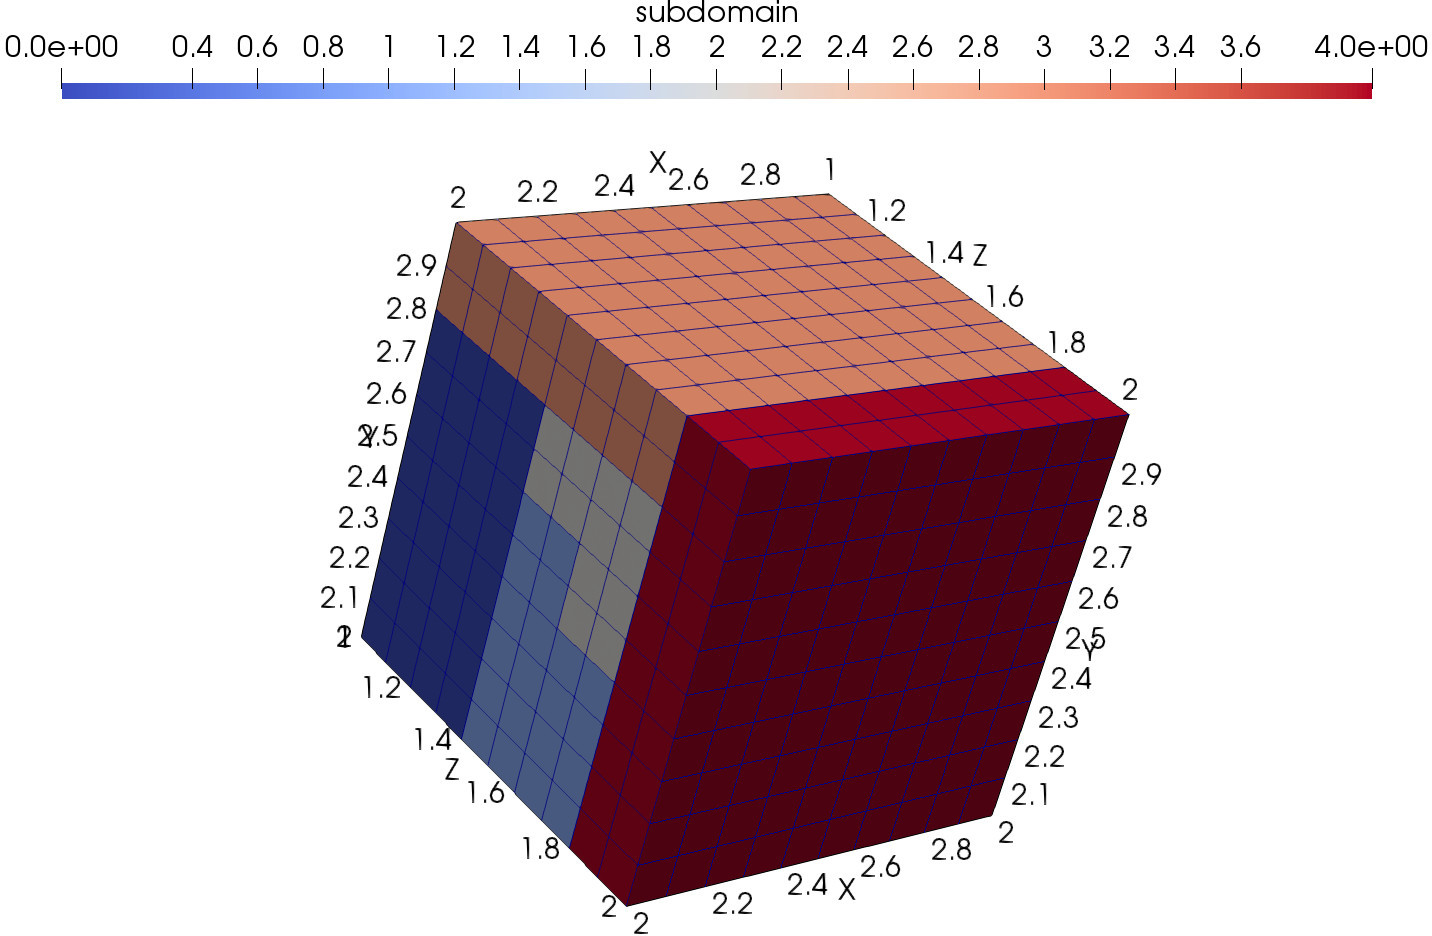
\includegraphics[width=0.78\textwidth]{img/mesh/cube.jpg}
			\vspace{-2mm}
		\caption{Cubical domain $\Omega$ with color-coded processor-owned elements.}
		\label{figure:domainDecomposition}
		\end{center}
	\end{figure}\vspace{-5mm}
	
\begin{figure}[H]
		\begin{center}
			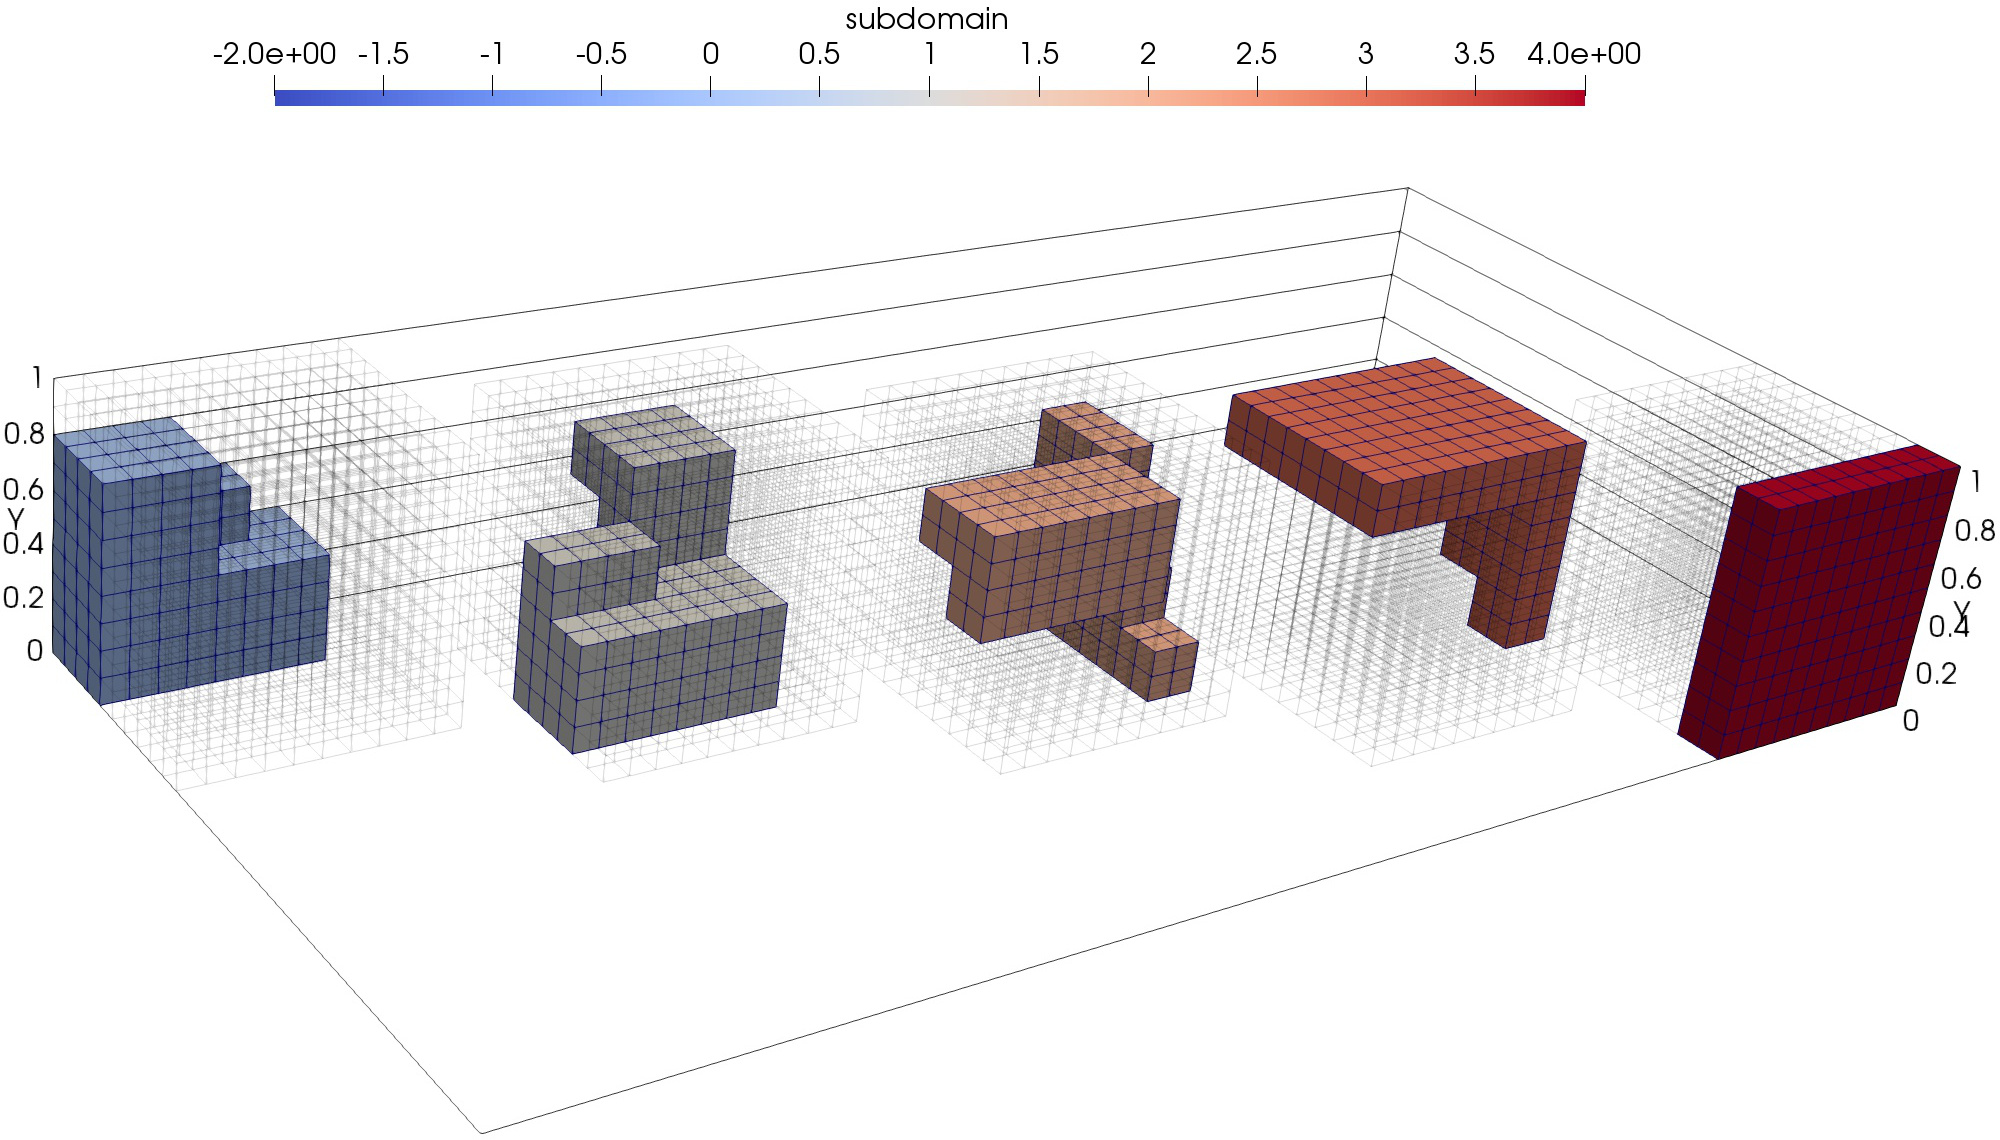
\includegraphics[width=0.78\textwidth]{img/mesh/cubeSub.jpg}
			\vspace{-2mm}
		\caption{The same domain as in \Cref{figure:domainDecomposition}, with clearer indication of elements that belong to individual processors (0..4 left to right).}
		\label{figure:domainDecomposition2}
		\end{center}
	\end{figure}\vspace{-5mm}
	

\section{Discontinuous Galerkin method}

For complex problems of compressible flow, and of course for even more complex problems of compressible MHD, there has been a number of attempts to use standard and well known Finite Element Methods that replace the spaces defined in \ref{Bochner} with finite-dimension spaces with bases formed by continuous piecewise polynomial functions. These attempts struggled with a common problem of spurious oscillations appearing in the solution - the origin of which is the lack of "stabilization", provided by the second-order terms in elliptic equations. Solution to these problems is the application of stabilization techniques, that usually introduce some sort of artificial diffusion (the second-order term), all of which are non-physical, and generally involve "magical" numbers - constants that are of pure computational nature (not a part of the physical description) or even worse are problem-specific.

\subsection{Overview of the DG method}
Due to this reason, there  was an effort to develop methods which would not need such stabilization techniques, and would still offer reasonable resolution of shockwaves, boundary and interior layers, and steep gradients without exhibiting spurious oscillations in the approximate solutions. The approach taken here is based on the idea to combine finite volume and Finite element methods leading to the so-called \emph{discontinuous Galerkin finite element method (DGFEM, DG)}. Here we shall derive and analyze DG for our equations. Let $T_h$ be a triangulation of $\Omega$. For each $K\in T_h$ we introduce the notation
\begin{eqnarray}
\partial K^- & = & \left\{x\in\partial K;\beta\lo\bs{x}\ro\cdot\bfn\lo\bs{x}\ro <0\right\},\\
\partial K^+ & = & \left\{x\in\partial K;\beta\lo\bs{x}\ro\cdot\bfn\lo\bs{x}\ro \geq 0\right\}.
\end{eqnarray}
By $H^1\lo\Omega, T_h\ro$ we denote the so-called \textit{broken Sobolev space}:
\be
\label{BrokenSobolev} H^1\lo\Omega,T_h\ro = \left\{v\in L^2\lo\Omega\ro;\ v|_K\in H^1\lo K\ro \forall K\in T_h\right\}.
\ee
This space is an approximation of the space defined in \ref{Sobolev}, but it contains functions that are discontinuous on element interfaces $\Gamma_ij$.
\paragraph{}
For $u\in H^1\lo\Omega,T_h\ro$ we set
\be
\label{PlusDef} u_K^+ = \text{trace of } u|_K \text{ on }\partial K
\ee
(i.e. the interior trace of $u$ on $\partial K$). For each face $E\subset\partial K\backslash\Gamma$ of $K$, there exists $K'\neq K,\ K'\in T_h$, adjacent to $E$ from the opposite side than $K$. Then we put
\be
\label{MinusDef} u_K^- = \text{trace of } u|_{K'} \text{ on } E.
\ee
In this way we obtain the exterior trace $u_K^-$ of $u$ on $\partial K\backslash\Gamma$ and define the jump of $u$ on $\partial K\backslash\Gamma$:
\be
[u]_K = u_K^+ - u_K^-.
\ee
\subsubsection{Approximation of the broken Sobolev space}
\label{section:Vh}
Let the domain $\Omega$ be covered with a mesh $T_h = 
\{ K_1,$ $K_2, \dots, K_M \}$ where each element $K_m$ carries an arbitrary
polynomial degree $1 \leq p_m$, $\forall m = 1, 2, \dots, M$. The broken Sobolev space 
$H^1\lo\Omega,T_h\ro$ will be approximated by a finite-dimensional space of picewise-polynomial functions
\be
\label{VH} V_{h} = \{ v \in L^2(\Omega); \ v|_{K_m} \in P^{p_m}(K_m)\ \mbox{for all}\ 1 \leq m \leq M \}
\ee
where $P^{p}$ is defined as
\bd
P^{p} = \mbox{span}\{\sum_{\substack{0\leq i, j, k \leq p \\i+j+k\leq p}}\alpha_i\ x_1^i\ x_2^j\ x_3^k,\ \ \alpha_i\in\mathbb{R} \}.
\ed

\subsection{DG formulation of MHD equations}
Although the resulting system will look very similar to the weak formulation \ref{WeakFinal}, the derivation makes more sense to be done starting with the \ref{conservativeGeneric}.
\paragraph{}
As stated in \ref{section:triangulation}, at this point we will discretize the problem in space, and leave the time-derivative untouched.
The approximate solution will be sought at each time instant $t$ as an element of the finite-dimensional space
$$
\left[V_h\right]^8,
$$
where $V_h$ is defined in \ref{VH}. Functions
$$
\mrvh \in \left[V_h\right]^8\approx \left[H^1\lo\Omega,T_h\ro\right]^8,
$$
where $H^1\lo\Omega,T_h\ro$ is defined in \ref{BrokenSobolev}, are in general discontinuous on interfaces $\Gamma_{ij}$.
By $\mrvh|_{ij}$ and $\mrvh|_{ji}$ we denote the values of $\mrvh$ on $\Gamma_{ij}$ considered from the
interior and the exterior of $K_i$, respectively. The symbols
$$
\left<\mrvh\right>_{ij} = \frac12 \lo \mrvh |_{ij} + \mrvh |_{ji}\ro,\ \left[\mrvh\right]_{ij} = \mrvh |_{ij} - \mrvh |_{ji}
$$
denote the average and jump of a function $\mrvh$ on $\Gamma_{ij}$.
In order to derive the discrete problem, we multiply \ref{conservativeGeneric} by a test function $\mrvh \in \left[V_h\right]^8$ in a component-wise fashion, integrate over any element $K_i \in T_h$, apply Green's theorem and sum over all $i \in I$, where $I$ is defined in \ref{Idef}:
\be
\label{DG1} \int_{\Omega_{t}} \pds{{\mrPsi_h}}{t} \mrvh - \sum_{K_i \in T_h}\int_{K_i}\mrF\lo{\mrPsi_h}\ro \lo\nabla \cdot \mrvh\ro + \sum_{K_i\in T_h} \sum_{j\in s_i} \int_{\Gamma_{ij}} \lo \mrF\lo{\mrPsi_h}\ro \cdot \bfn_{ij} \ro \mrvh = \int_{\Omega_{t}} \mrS \mrvh,
\ee
where $\bfn_{ij}$ is the unit outer normal to $\Gamma_{ij}$.
Now, the term
\be
\label{NonUniqueTerm} \int_{\Gamma_{ij}} \mrF\lo{\mrPsi_h}\ro \cdot \bfn_{ij} \mrvh
\ee
is problematic, because the value of ${\mrPsi_h}$ on $\Gamma_{ij}$ is not unique - we have two values:
\begin{itemize}
    \item ${\mrPsi_h}|_{ij}$ - which is the value of ${\mrPsi_h}$ on $\Gamma_{ij}$ considered from the element $K_i$,
    \item ${\mrPsi_h}|_{ji}$ - which is the value of ${\mrPsi_h}$ on $\Gamma_{ij}$ considered from the element $K_j$.
\end{itemize}
\textbf{Note: }This corresponds to the notation set in \ref{PlusDef}, \ref{MinusDef} - if we take $K_i$ as the element at hand, we have
$$
{\mrPsi_h}|_{ij} = {\mrPsi_h}_{K_i}^+,\ \ {\mrPsi_h}|_{ji} = {\mrPsi_h}_{K_i}^-
$$
\paragraph{}
Now, because of this non-uniqueness of the values, we replace the term \ref{NonUniqueTerm} with the so-called \textit{numerical flux} $\mrH = \mrH\lo\mrvh, \mrw, \bfn\ro$ in the following fashion:
\be
\label{NumFluxDef}
\lo\mrF\lo{\mrPsi_h}\ro \cdot \bfn_{ij}\ro \mrvh \approx \mrH\lo{\mrPsi_h}|_{ij}, {\mrPsi_h}|_{ji}, \bfn_{ij}\ro \mrvh.
\ee
We impose the following requirements on the numerical flux:
\begin{enumerate}
	\item $\mrH\lo \mrvh, \mrw, \bfn\ro$ is defined and continuous on $\mc{D} \times \mc{D} \times \mc{S}_1$, where $\mc{D}$ is the domain of definition of the flux $\mrF$ and $\mc{S}_1$ is the unit sphere in $\mathbb{R}^3$.
	\item $\mrH$ is $consistent$:
		\be
			\label{FluxConsistent} \mrH\lo \mrvh, \mrvh, \bfn\ro = \mrF\lo \mrvh\ro \bfn,\ \mrvh\in\mc{D},\ \bfn\in\mc{S}_1.
		\ee
	\item $\mrH$ is $conservative$:
		\be
			\label{FluxConservative} \mrH\lo \mrvh, \mrw, \bfn\ro = -\mrH\lo \mrw, \mrvh, -\bfn\ro,\ \mrvh, \mrw\in\mc{D},\ \bfn\in\mc{S}_1.
		\ee
 \end{enumerate}
It follows from \ref{NumFluxDef}, that the numerical flux can be seen as the solution of the 1-dimensional \textit{Riemann problem}:
\begin{eqnarray}
\mrU & = & \lo\begin{array}{c}\rho \\ \pi_1 \\ \pi_2 \\ \pi_3 \\ U \\ B_2 \\ B_3 \\ \end{array}\ro,\ \mrF = \lo\begin{array}{c} \pi_1 \\ \frac{\pi_1^2}{\rho} - B_1^2 + \frac12\lo p + U_m\ro \\ \frac{\pi_2 \pi_1}{\rho} - B_1 B_2 \\ \frac{\pi_3 \pi_1}{\rho} - B_1 B_3\\ \frac{\pi_1}{\rho} \lo \frac{\gamma}{\gamma - 1} p + U_k\ro + \frac{2}{\rho} \lo \pi_k B_1 - \pi_1 B_k\ro B_1  \\ \frac{\pi_1 B_2 - \pi_2 B_1}{\rho} \\ \frac{\pi_1 B_3 - \pi_3 B_1}{\rho} \\ \end{array}\ro.
\end{eqnarray}

And using these properties of the numerical flux, we can rewrite \ref{DG1} as:
\begin{eqnarray}
\label{DG2} \int_{\Omega_{t}} \pds{{\mrPsi_h}}{t} \mrvh & - & \sum_{K_i \in T_h}\int_{K_i}\mrF\lo{\mrPsi_h}\ro \lo\nabla \cdot \mrvh\ro\\ \nonumber & + & \sum_{\Gamma_{ij}\in\Gamma_I} \int_{\Gamma_{ij}} \mrH\lo{\mrPsi_h}|_{ij}, {\mrPsi_h}|_{ji}, \bfn_{ij}\ro \mrvh = \int_{\Omega_{t}} \mrS \mrvh,
\end{eqnarray}
where we used the definition of \ref{InternalEdges} on the page \pageref{InternalEdges}.
\subsection{Numerical flux}
Generally, the numerical flux function can be a non-differentiable (or even discontinuous) function. That is challenging from the perspective of the usage of Newton's method to solve the resulting nonlinear problem arising when using implicit time-discretization.\ \\
Another complication arising from evaluation of numerical fluxes on element interfaces exists in distributed solver, where we need to make sure that all processors have relevant data (e.g. previous solution values) from all cells that neighbor any cells assembled on the processor at hand. This issue gets worse when local mesh refinement (there are more neighbor elements of the current cell across the interface at hand), as well as if periodic boundary conditions are used (the neighbor graph is more complex).
\subsubsection{Riemann problem for MHD}
The flux matrix of the MHD equations in one (x-) dimension (where, due to the divergence free condition $\nabla\cdot \bfB = 0$ of the magnetic field), $B_1$ is given as constant, have seven eigenvalues which correspond to two Alfve'n waves ($\lambda_{2, 6}$), two slow magneto-acoustic waves ($\lambda_{3, 5}$), and two fast magneto-acoustic waves ($\lambda_{1, 7}$), and one entropy wave ($\lambda_{4}$):
\begin{eqnarray}
\lambda_{2, 6} = \frac{\pi_1}{\rho} \mp c_a,\\
\lambda_{3, 5} = \frac{\pi_1}{\rho} \mp c_s,\\
\lambda_{1, 7} = \frac{\pi_1}{\rho} \mp c_f,\\
\lambda_{4} = \frac{\pi_1}{\rho},
\end{eqnarray}
where $c_a = \sqrt{\frac{B_1^2}{rho}}$, $c_{s, f} = \left\{\frac{\gamma p + |B|^2 \mp \sqrt{\left(\gamma p + |B|^2\right)^{\frac12} - 4\gamma p B_1^2}}{2\rho}\right\}^{\frac12}$.
\paragraph{}
For MHD equations, there is no exact solver of the Riemann problem across the element boundary, and approximate solvers are used. The fluxes chosen are listed further.
\subsubsection{Lax-Friedrichs numerical flux}
This is the most straightforward numerical flux satisfying \ref{FluxConsistent}, and \ref{FluxConservative} and is defined as follows:
\be
,
\ee
where the parameter $\alpha$ is the so-called \textit{stabilization parameter}, usually having value $\alpha = 0.5$. Now, this numerical flux is very diffusive (TODO citace), and is only used for implementation verification purposes, as due to its simplicity, the risk of errors in the implementation is rather negligible.
\subsubsection{HLLD numerical flux}
The abbreviation \textbf{HLLD} stands for Harten-Lax-van Leer (HLL) approximate Riemann solver, and \textbf{D} stands for Discontinuities.
This particular numerical flux has been introduced in \citep{hlld} and has been shown to be very suitable for the studied problems.
TODO: doplnit
\subsection{Numerical handling of boundary conditions}
In what follows, we are only interested in using flux-induced inflow and outflow boundary conditions (see Section \ref{section:bcs}).
To account for these boundary conditions, we need to investigate the term
$$
\int_{\Gamma_{ij}} \mrH\lo{\mrPsi_h}|_{ij}, {\mrPsi_h}|_{ji}, \bfn_{ij}\ro \mrvh
$$
for $\Gamma_{ij} \in \Gamma_B$ (see \ref{BndEdges} on page \pageref{BndEdges}).
This term is used in \ref{DG2} for faces in $\Gamma_I$ which are internal and always have 2 values connected to them - $\mrPsi_h|_{ij}, {\mrPsi_h}|_{ji}$ - which induces the notation. On a boundary face, the corresponding value to ${\mrPsi_h}|_{ij}$ can be defined correspondingly as in the case of $\Gamma_I$, but ${\mrPsi_h}|_{ji}$ needs to be defined.
\subsubsection{Inflow boundary condition}
First, if we want to prescribe an inflow boundary condition (i.e. we know what values should the state vector $\mrPsi_h$ have on ${\Gamma_{ij}}\in\Gamma_B$), we define
\be
\label{BC1} \overline{{\mrPsi_h}|_{ji}}
\ee
to be the prescribed value.

\subsubsection{Outflow boundary condition}
If we want to model an outflow boundary condition (i.e. do nothing condition), we may use the \textit{consistency} of the numerical flux $\mrH$ defined in \ref{FluxConsistent}, and define
\be
\label{BC2} \overline{{\mrPsi_h}|_{ji}} = {\mrPsi_h}|_{ij},
\ee
which is a suitable definition for the outflow boundary condition. It is important to mention, that setting the inflow boundary condition does not imply that solution values on this boundary equal to these prescribed value. This follows from the definition of broken Sobolev space (\ref{BrokenSobolev}). Moreover the values of the solution on the boundary also depend on the numerical flux used, as the values on the boundary are merely one of the input parameters for the flux (See \ref{NumFluxDef}).

Now, taking \ref{BC1} and \ref{BC2}, we can enhance \ref{DG2} with an additional term, that will add the boundary conditions into the equation:
$$
\sum_{\Gamma_{ij}\in\Gamma_B} \int_{\Gamma_{ij}} \mrH\lo{\mrPsi_h}|_{ij}, \overline{{\mrPsi_h}|_{ji}}, \bfn_{ij}\ro \mrvh,
$$
so that the complete semi-discrete problem reads:
\begin{eqnarray}
\label{DG3} \int_{\Omega_{t}} \pds{{\mrPsi_h}}{t} \mrvh & - & \sum_{K_i \in T_h}\int_{K_i}\mrF\lo{\mrPsi_h}\ro \lo\nabla \cdot \mrvh\ro\\ \nonumber & + & \sum_{\Gamma_{ij}\in\Gamma_I} \int_{\Gamma_{ij}} \mrH\lo{\mrPsi_h}|_{ij}, {\mrPsi_h}|_{ji}, \bfn_{ij}\ro \mrvh\\\nonumber
 & + & \sum_{\Gamma_{ij}\in\Gamma_B} \int_{\Gamma_{ij}} \mrH\lo{\mrPsi_h}|_{ij}, \overline{{\mrPsi_h}|_{ji}}, \bfn_{ij}\ro \mrvh\\\nonumber
 & = & \int_{\Omega_{t}} \mrS \mrvh.
\end{eqnarray}

\paragraph{}
Now we can formulate the definition of the \textit{semi-discrete solution ${\mrPsi_h} = {\mrPsi_h}\lo(t, \bfx\ro)$ of MHD equations \ref{conservativeGeneric}} as
\begin{enumerate}
    \label{discreteSlnDef}
    \item ${\mrPsi_h} \in C^{1}\lo\lo0, T\ro, \left[V_h\right]^8\ro$,
    \item \ref{DG3} holds for all $t\in\lo0, T\ro$, and all $\mrv\in \left[V_h\right]^8$,
    \item ${\mrPsi_h}\lo0, \bfx\ro = \Pi_h \mrPsi^0\lo\bfx\ro$,
\end{enumerate}
where $\Pi_h$ is a projection of the initial condition $\mrPsi^0$ onto $\left[V_h\right]^8$.




\section{Divergence-free FE space}
The divergence-free constraint of the magnetic field, $\bfB = 0$ (Gauss's law) is not enforced by the solution definition \ref{weakSlnDef}. Therefore, we need to perform additional work to be sure that we do not have a non-physical solution in the sense that the constraint is not satisfied.
\paragraph{}
There are two often used approaches to handle this problem - the Constraint-Transport (CT) method, and divergence cleaning. The first one is not suitable for this work, as it constraints the triangulation in such a way, that implementing Adaptive Mesh Refinement would be very complicated, if possible at all. The second approach, the divergence cleaning methods need additional postprocessing step which may be omitted for the sake of calculation efficiency. The approach taken in this work is to replace the standard FE space  \ref{feSpaceDef} with basis functions \ref{feSpaceBasis} for the magnetic field part ($B$) with a vector-valued (3-dimensional) space $V_h^B$ of functions that have exactly
\be
\nabla \cdot \mrvh^B = 0,\ \ \mrvh^B\in V_h^B,
\ee
where these functions are as before discontinuous on interfaces $\Gamma_{ij}$.
The basis of space $V_h^B$ for piecewise-linear functions can be selected in several ways, in this work, the following basis was selected:
\begin{table}[H]
	\begin{tabular*}{\textwidth}{cccc}
\hline
\\
		$\lo\begin{array}{c}B_x\lo x, y, z\ro\\B_y\lo x, y, z\ro\\B_z\lo x, y, z\ro \end{array}\ro$ & Visualization & $\lo\begin{array}{c}B_x\lo x, y, z\ro\\B_y\lo x, y, z\ro\\B_z\lo x, y, z\ro \end{array}\ro$ & Visualization \\ 
\\
		\hline
		\\
\end{tabular*}
	\begin{tabular*}{\textwidth}{cccc}
	$\lo\begin{array}{c}1\\0\\0 \end{array}\ro$ & \raisebox{-0.5\totalheight}{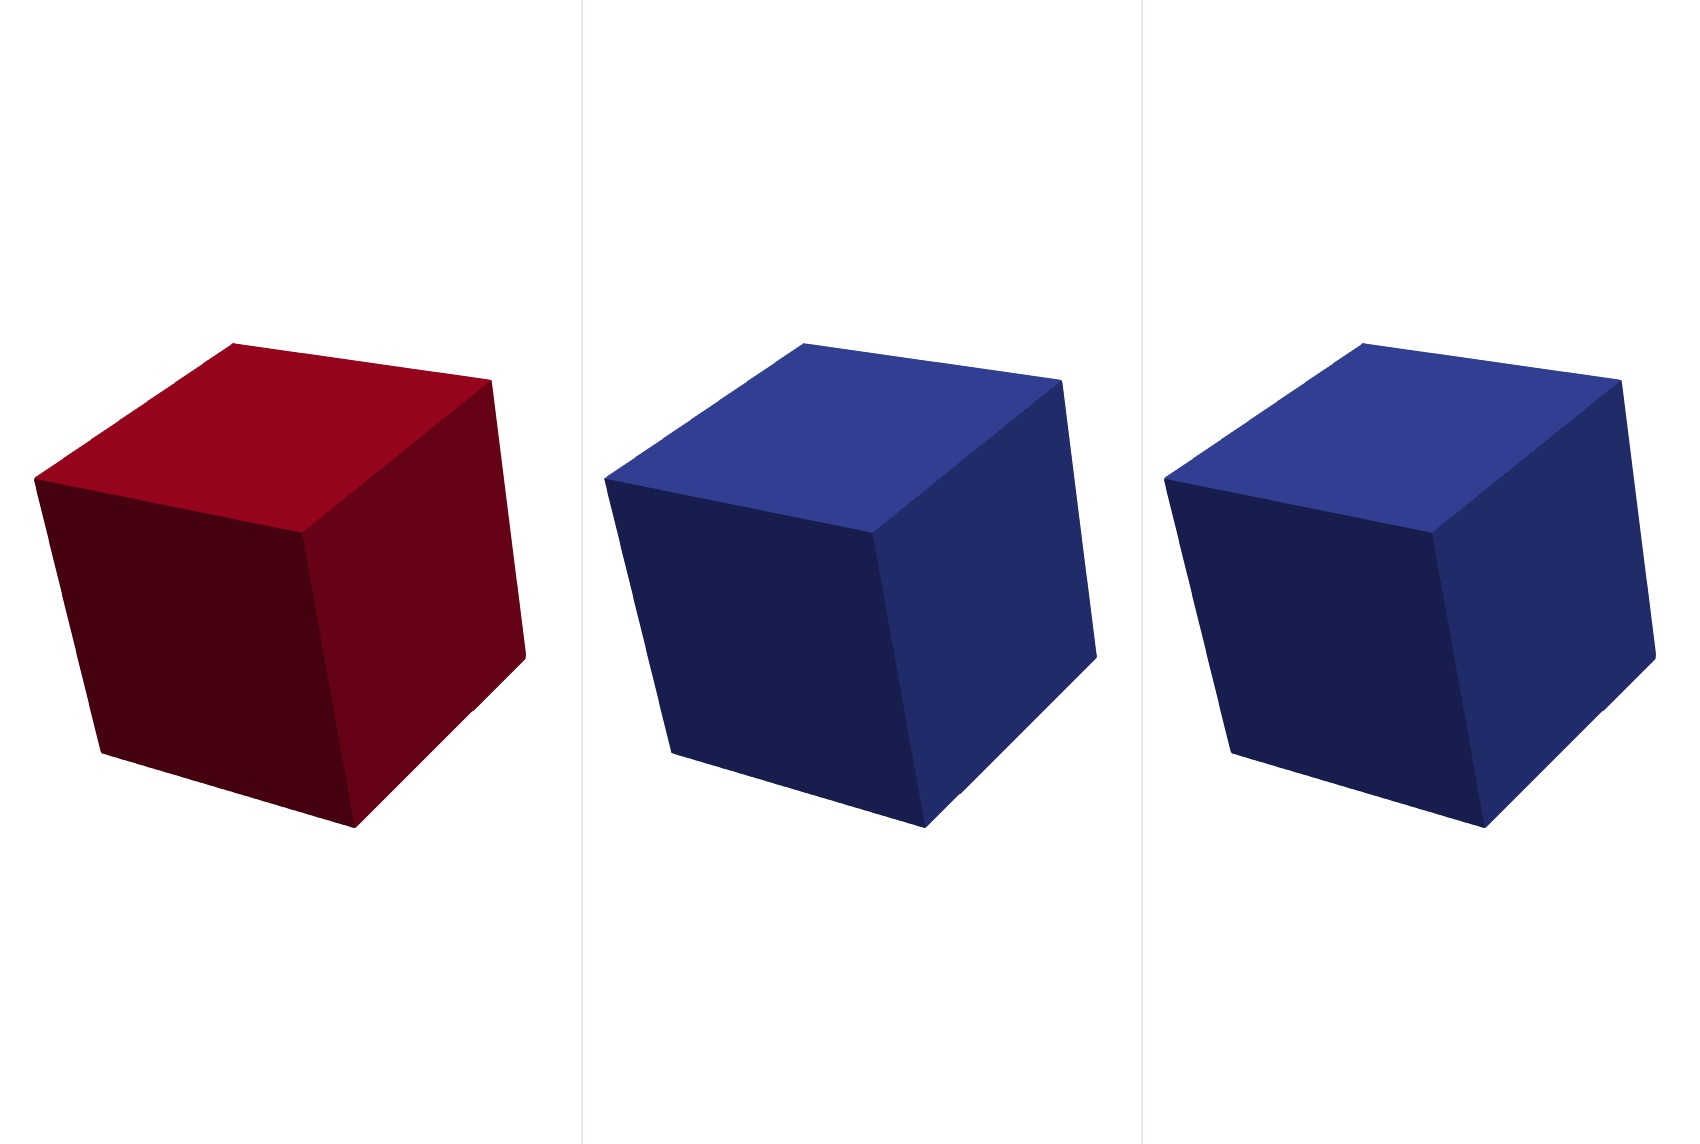
\includegraphics[width=0.3\textwidth]{img/basis/1.jpg}} & $\lo\begin{array}{c}0\\0\\y \end{array}\ro$ & \raisebox{-0.5\totalheight}{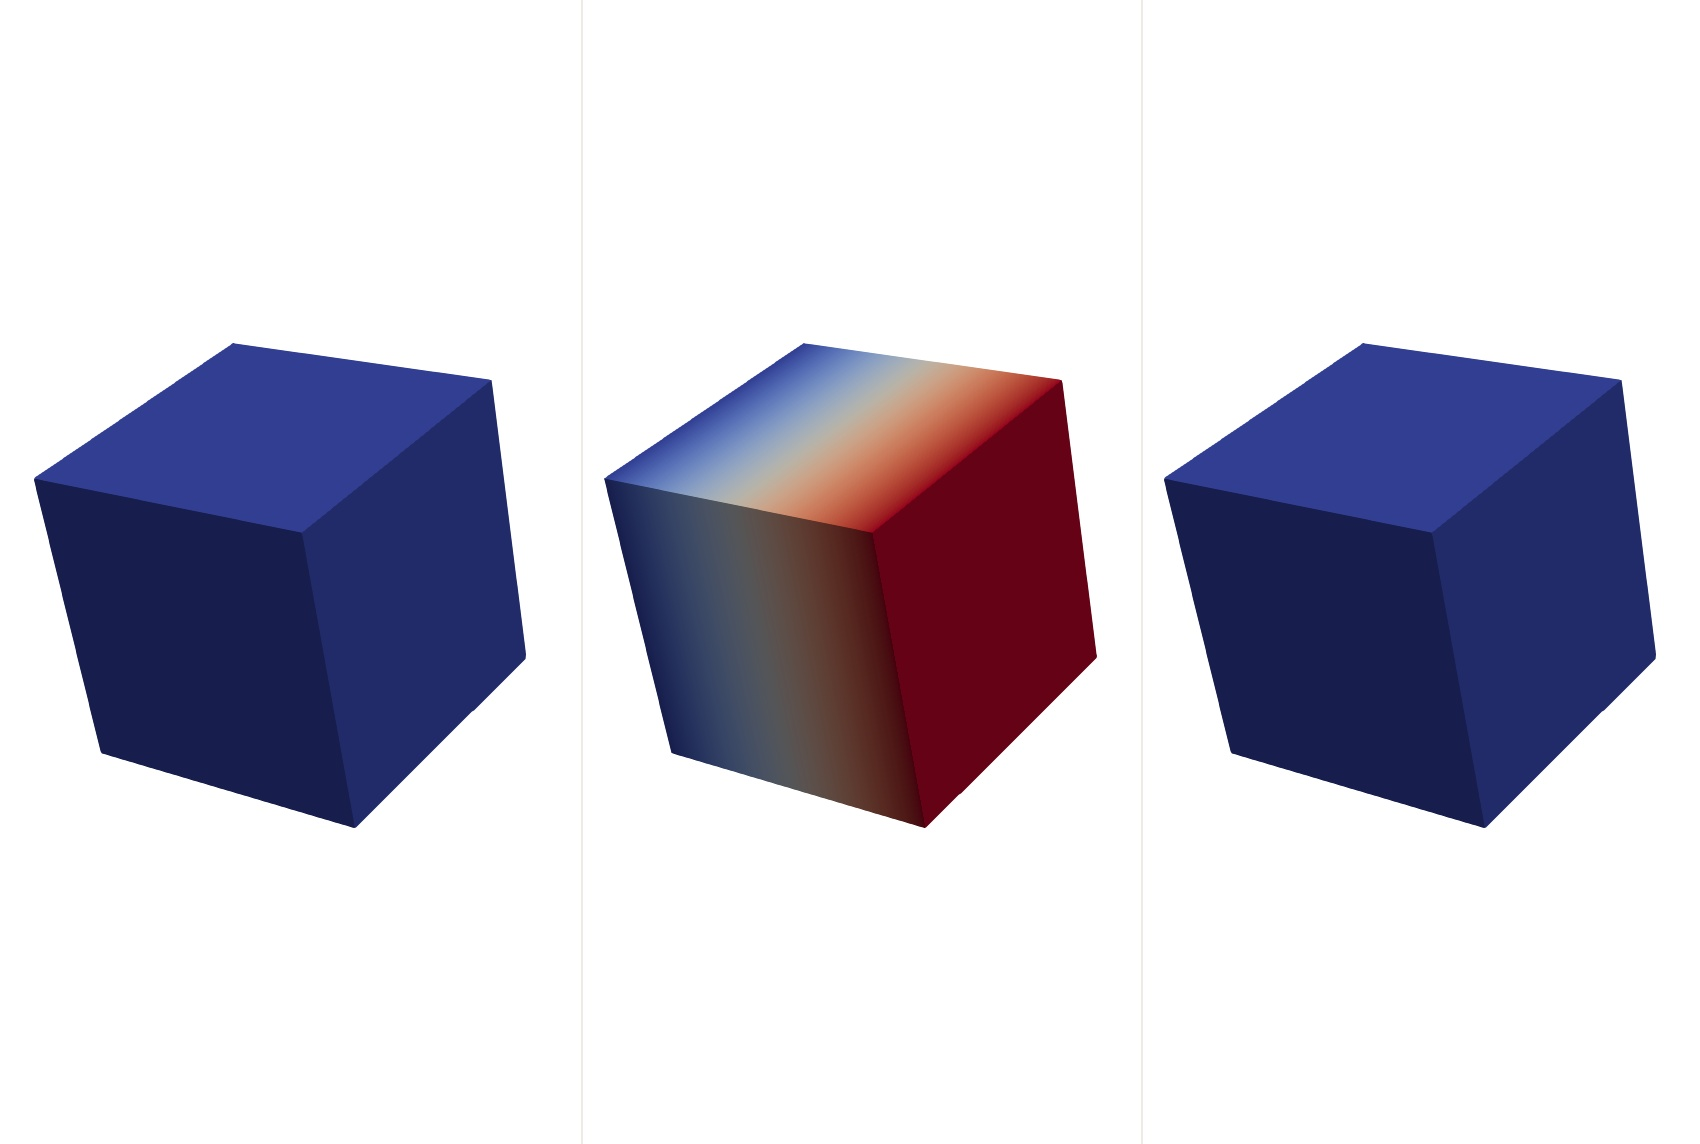
\includegraphics[width=0.3\textwidth]{img/basis/6.jpg}}\\
	\\	
	$\lo\begin{array}{c}0\\1\\0 \end{array}\ro$ & \raisebox{-0.5\totalheight}{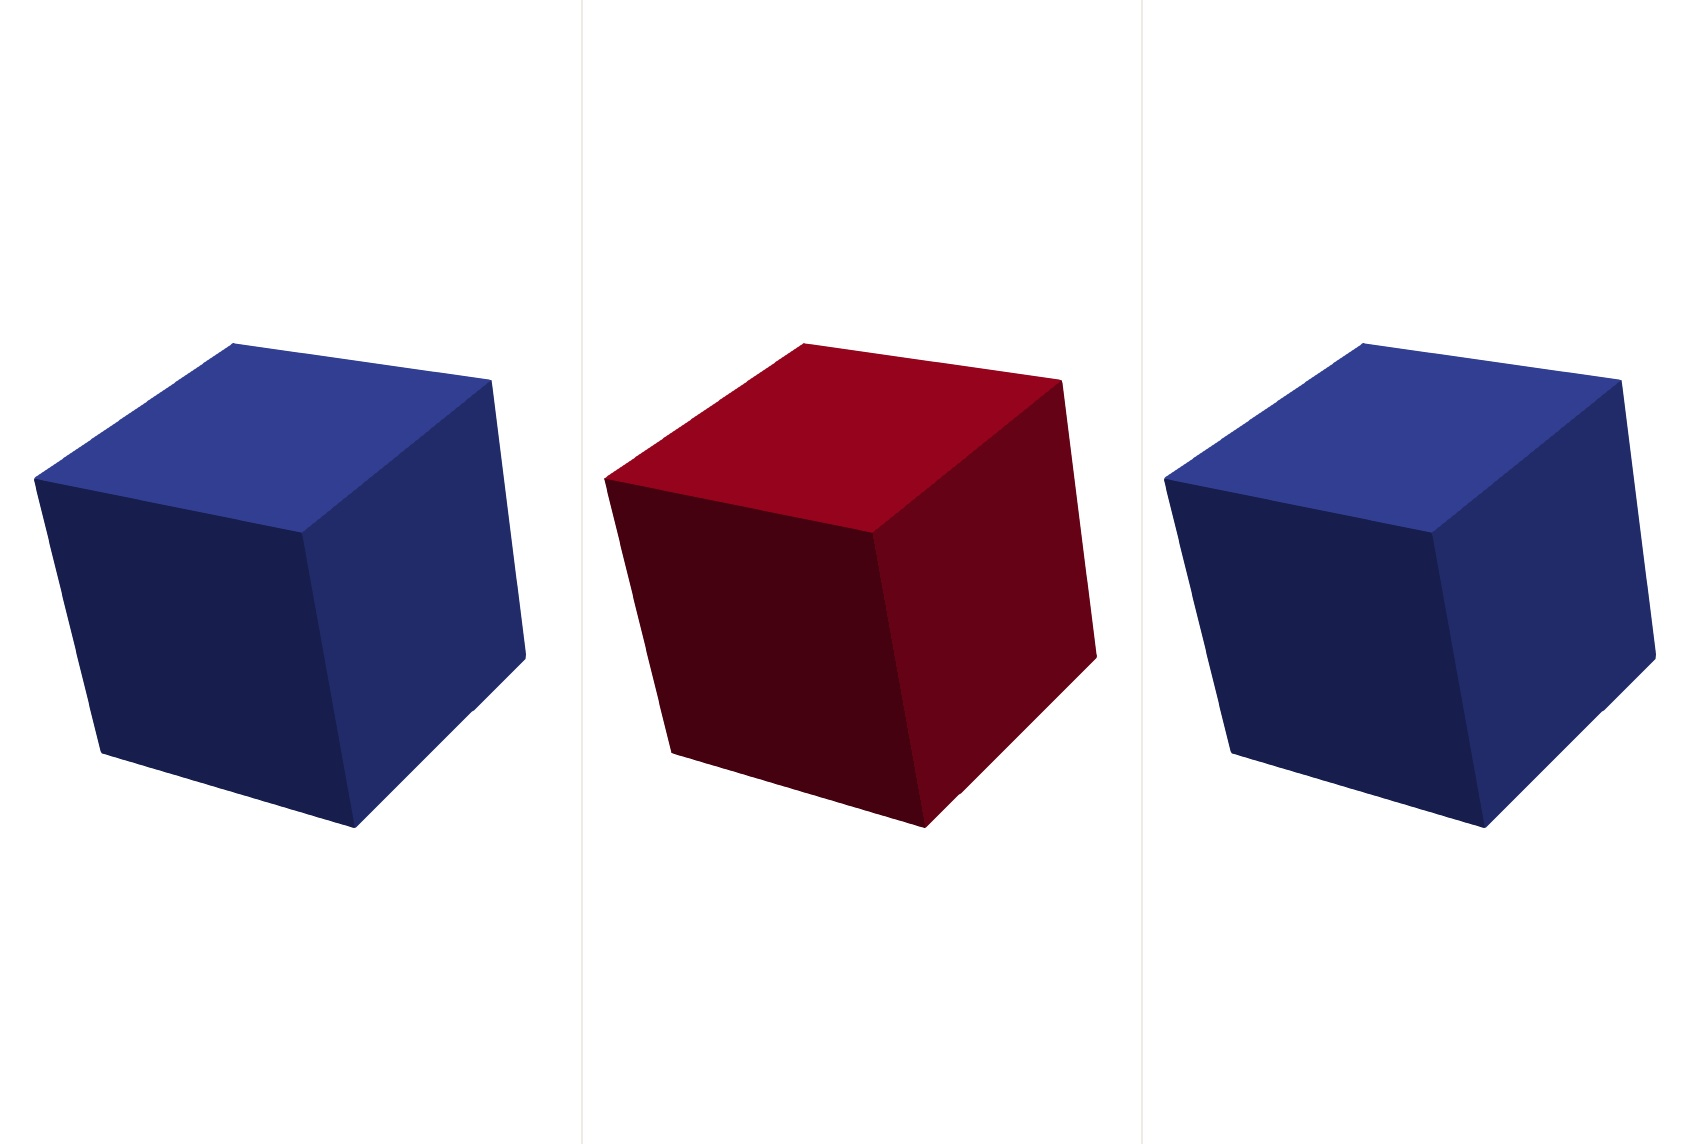
\includegraphics[width=0.3\textwidth]{img/basis/2.jpg}} & $\lo\begin{array}{c}z\\0\\0 \end{array}\ro$ & \raisebox{-0.5\totalheight}{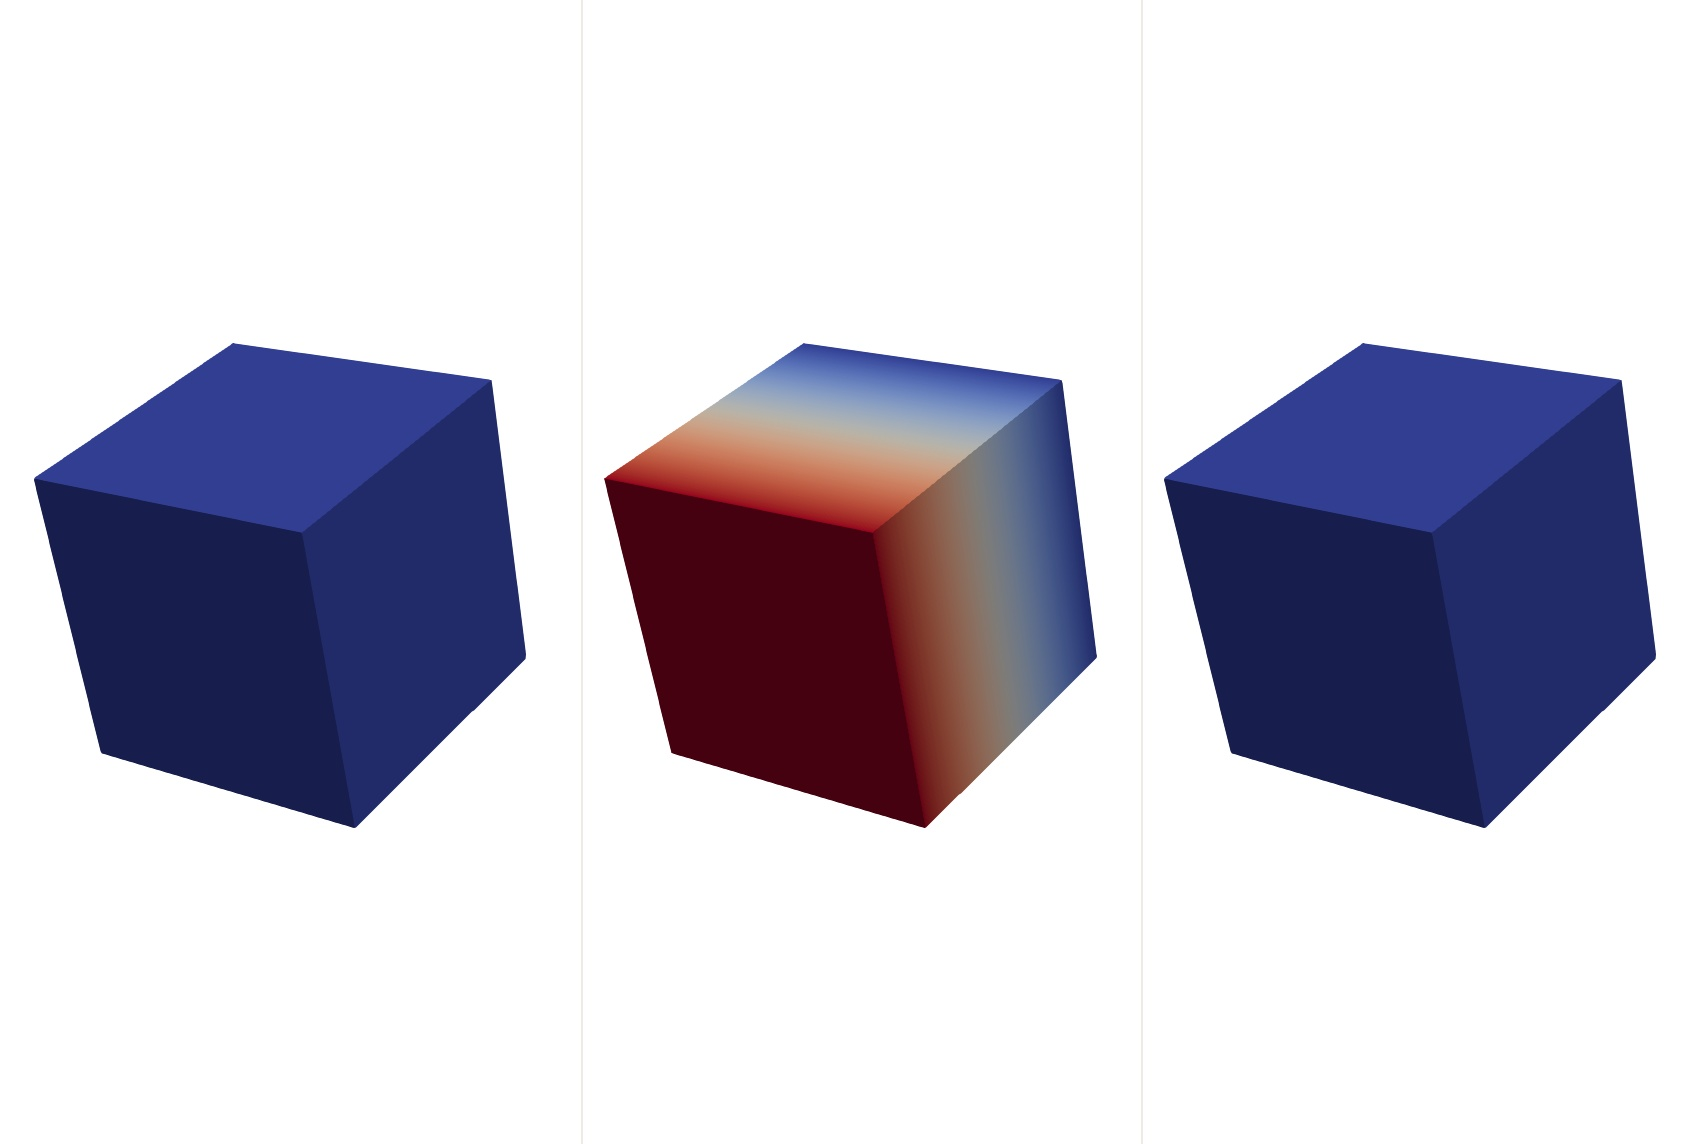
\includegraphics[width=0.3\textwidth]{img/basis/7.jpg}}\\
		\\	
	$\lo\begin{array}{c}0\\0\\1 \end{array}\ro$ & \raisebox{-0.5\totalheight}{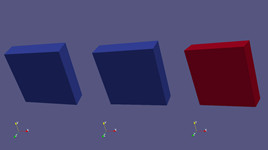
\includegraphics[width=0.3\textwidth]{img/basis/3.jpg}} & $\lo\begin{array}{c}0\\z\\0 \end{array}\ro$ & \raisebox{-0.5\totalheight}{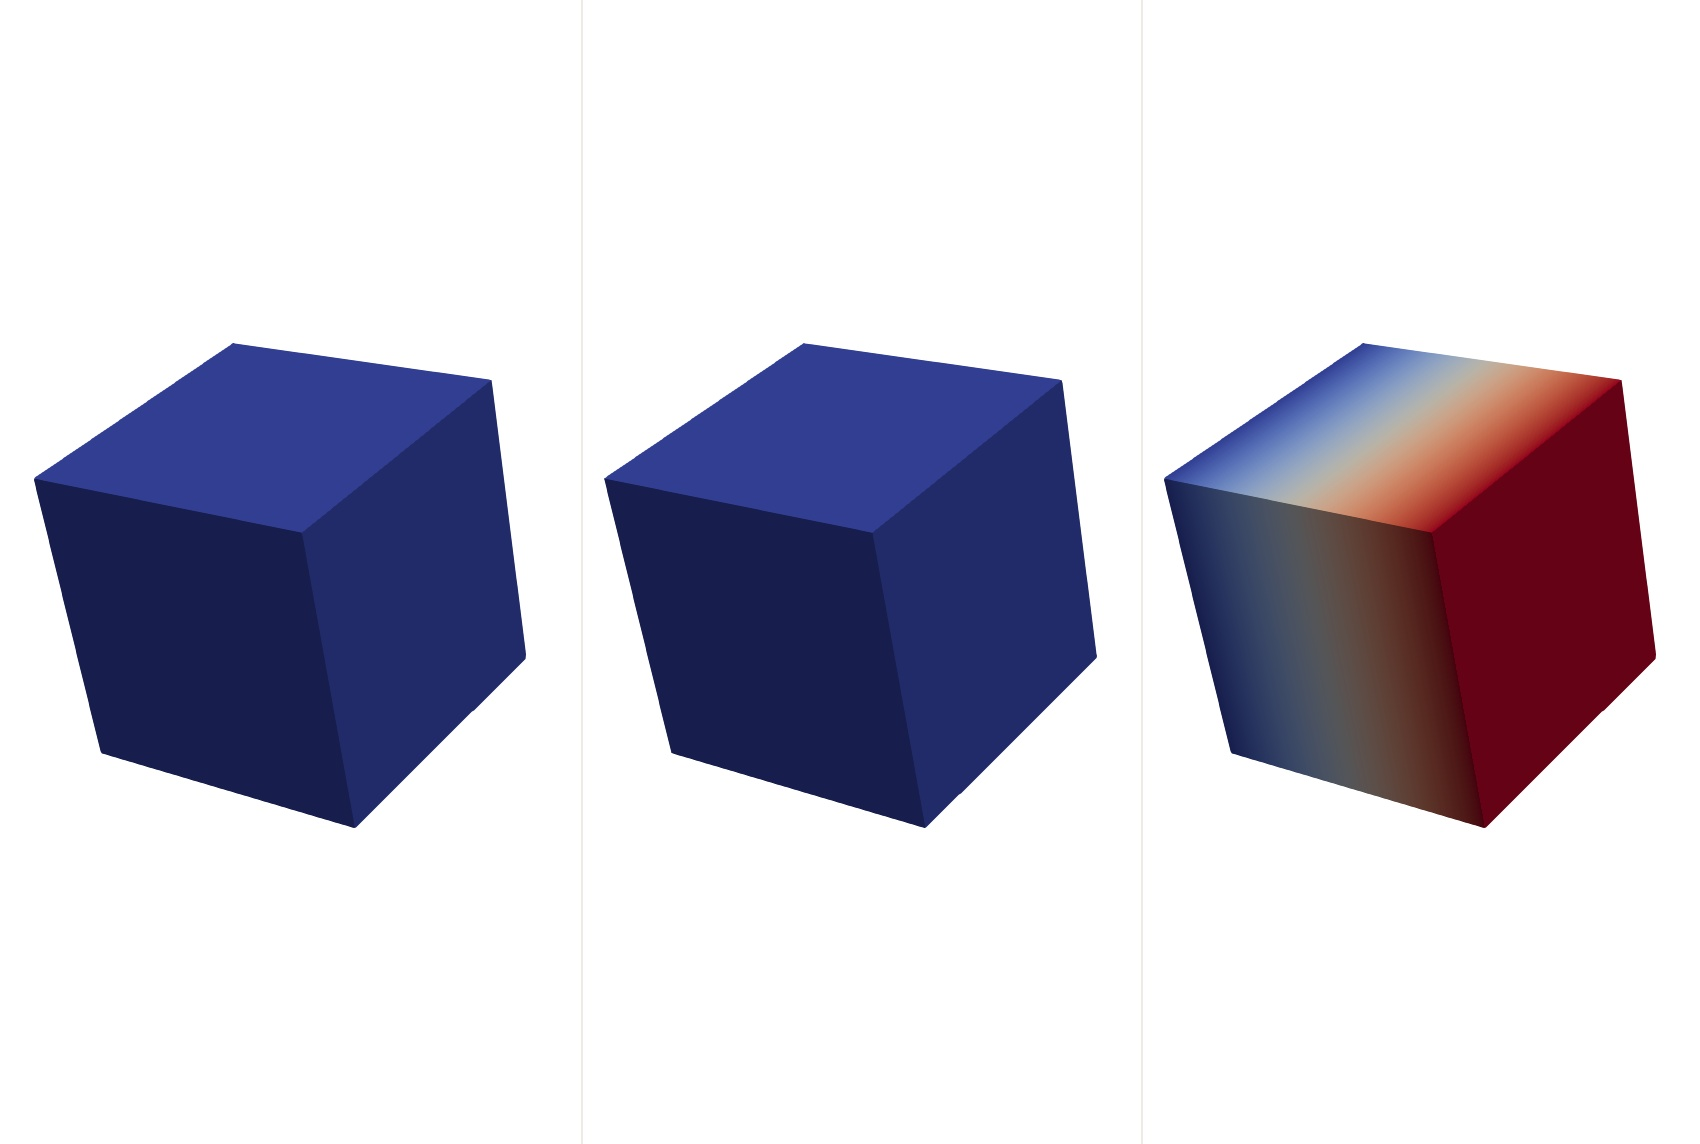
\includegraphics[width=0.3\textwidth]{img/basis/8.jpg}}\\
		\\	
	$\lo\begin{array}{c}y\\0\\0 \end{array}\ro$ & \raisebox{-0.5\totalheight}{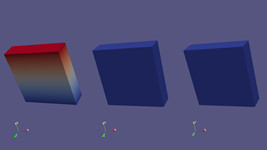
\includegraphics[width=0.3\textwidth]{img/basis/4.jpg}} & $\lo\begin{array}{c}0\\0\\x \end{array}\ro$ & \raisebox{-0.5\totalheight}{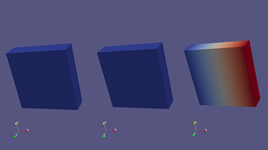
\includegraphics[width=0.3\textwidth]{img/basis/9.jpg}}\\
		\\	
	$\lo\begin{array}{c}0\\x\\0 \end{array}\ro$ & \raisebox{-0.5\totalheight}{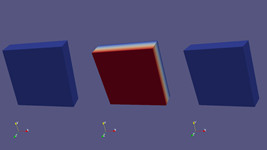
\includegraphics[width=0.3\textwidth]{img/basis/5.jpg}} & $\lo\begin{array}{c}2x\\-y\\-z \end{array}\ro$ & \raisebox{-0.5\totalheight}{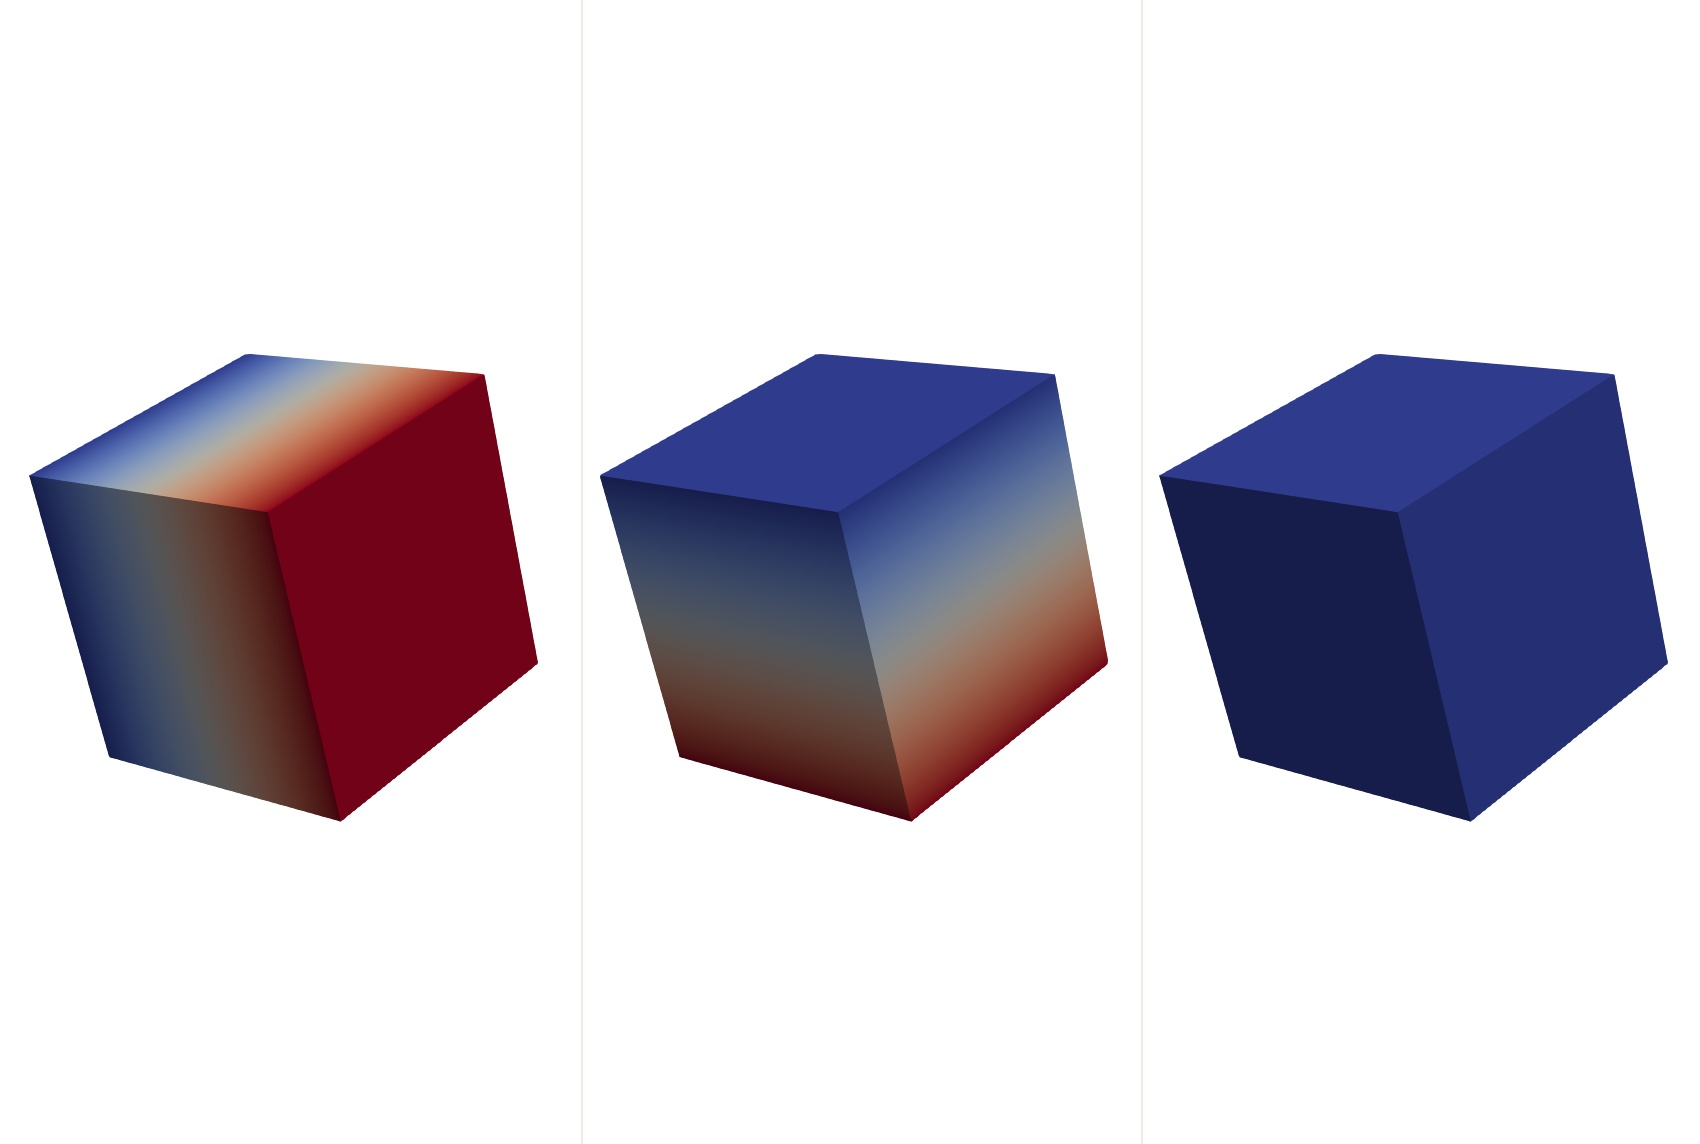
\includegraphics[width=0.3\textwidth]{img/basis/10.jpg}}\\	
	\\	
			\hline		
		\end{tabular*}
		\caption{Divergence-free space basis}
	\label{tbl:divFreeBasis}
\end{table}
In \ref{tbl:divFreeBasis}, it is obvious that only one function actually has more nonzero components.
\paragraph{}
In what follows, the notation $\left[V_h\right]^8$ used before will be used for the space where the last three components are replaced by $V_h^B$. Note that there are some technicalities with respect to the usage of $V_h^B$ needed to be handled in computation, e.g. in \ref{vertexBasedAlpha}, or later in \ref{Final_Integration_Fn}, \ref{Final_Integration_Fn_b} that we do not explicitly attend to.

\section{Discretization in time}
Relations \Cref{DG2} represent a system of ordinary differential equations which can be solved by a suitable numerical method. Since we are interested in applying the Rothe's method (as opposed to the method of lines, which switches the order of discretization in time and space), we now want to discretize the time derivative. In order to do so, we consider a partition $0 = t_0 < t_1 < t_2 < ...$ of the time interval $\lo 0, T\ro$ and set $\tau_k = t_{k+1} - t_k$. We use the notation $\bfw_h^k$ for the approximation of $\bfw_h\lo t_k\ro$.

\subsection{Discrete problem}
\label{section:discreteProblem}
Then we apply a time discretization scheme, for example, the simple explicit \emph{Euler method} and our \emph{fully discrete problem} reads: for each $k > 0$ find $\bfw_h^{k+1}$ such that
\begin{enumerate}
    \item ${\mrPsi_h}^{k+1} \in \left[V_h\right]^8$,
    \item For all test functions $\mrvh\in\left[V_h\right]^8$:
			\begin{align}
			\label{DiscretizedFull} \int_{\Omega_{t}} \frac{{\mrPsi_h}^{k+1} - {\mrPsi_h}^{k}}{\tau} \mrvh & - \sum_{K_i \in T_h}\int_{K_i}\mrF\lo{\mrPsi_h^{k}}\ro \lo\nabla \cdot \mrvh\ro\\
			\nonumber & + \sum_{\Gamma_{ij}\in\Gamma_I} \int_{\Gamma_{ij}} \mrH\lo{\mrPsi_h^{k}}|_{ij}, {\mrPsi_h^{k}}|_{ji}, \bfn_{ij}\ro \mrvh \\
			\nonumber & + \sum_{\Gamma_{ij}\in\Gamma_B} \int_{\Gamma_{ij}} \mrH\lo{\mrPsi_h^{k}}|_{ij}, \overline{{\mrPsi_h^{k}}|_{ji}}, \bfn_{ij}\ro \mrvh\\
			\nonumber & = \int_{\Omega_{t}} \mrS \mrvh,
			\end{align}
    \item ${\mrPsi_h}^{0}\lo\bfx\ro = \Pi_h \mrPsi^0\lo\bfx\ro$,
\end{enumerate}
where $\Pi_h$ is a projection of the initial condition $\mrPsi^0$ onto $\left[V_h\right]^8$.
\subsection{Time step length}
\label{section:CFL}
Time step length is an important attribute of the discretization. If it is too small, the calculation might be taking too long to finish, with unnecessary precision with respect to time. If it is too large, we may end up with unstable calculation and obtain results with nonphysical oscillations, or without a solution whatsoever. That is why we need to take extra care to derive the proper value. From the stability perspective, we have a condition for the upper bound of the time step - this condition is called the \textit{Courant-Friedrichs-Lewy} condition. This condition is of the following form:
\be
\label{CFLcond}
\tau_{max} = \text{min}\left\{\frac{{\Delta_{x}}_{min}}{c_{max}}, \frac{{\Delta_{x}}_{min}^2}{2 \eta_{max}}\right\},
\ee
where
${\Delta_{x}}_{min}$ is the smallest dimension of any element, $\eta_{max}$ highest resistivity in the domain, and $v_{max}$ highest velocity in the domain, where the following velocities are taken into account:
\begin{align}
c_s & =  \sqrt{\frac{\gamma\lo\gamma-1\ro}{\rho}\lo U - \rho v^2-U_B\ro},\\
c_a & =  \sqrt{\frac{B^2}{\rho}},\\
u,
\end{align}
where $c_s$ is the speed of sound, $c_a$ is the Alfv�n speed, and $u$ is the speed of plasma. We then take
$$
c_{max} = \text{max}\left\{c_s, c_a, u \right\}.
$$

\section{Algebraic formulation}
Last step in the DG method discretization is to transform the system of equations \Cref{DiscretizedLinear} into a system of linear algebraic equations at every time step $t_k$ and obtain the solution at this time step as the solution of this linear algebraic system.
\paragraph{}
First, we rearrange the system in the following manner:
\begin{align}
\label{RewrittenLinearSystem} \sum_{K_i \in T_h}\int_{K_i} \mrvh {\mrPsi_h}^{k+1} & = 
\sum_{K_i \in T_h}\int_{K_i} \left[{\mrPsi_h}^{k} + \tau\mrS + \tau\mrA\lo{\mrPsi_h^{k}}\ro \lo\nabla \cdot \mrvh\ro\right] \mrvh \\\nonumber& - \sum_{\Gamma_{ij}\in\Gamma_I} \int_{\Gamma_{ij}}\mrH\lo{\mrPsi_h^{k}}|_{ij}, {\mrPsi_h^{k}}|_{ji}, \bfn_{ij}\ro \mrvh
\\\nonumber& - \sum_{\Gamma_{ij}\in\Gamma_B} \int_{\Gamma_{ij}} \mrH\lo{\mrPsi_h^{k}}|_{ij}, \overline{{\mrPsi_h^{k}}|_{ji}}, \bfn_{ij}\ro \mrvh.
\end{align}
We can see that the left hand side does not depend on the previous solution values, so there is no need to recalculate the matrix entries in every time step (unless we employ AMR, in which case the mesh and therefore the set of basis functions changes).
Now
\be
\label{Coeffs} {\mrPsi_h}^{k+1} = \sum_{l = 0}^{l = L} y_l {\mrvh}_l, L = \mathrm{dim}\lo\left[V_h\right]^8\ro
\ee
for some (obviously finite) basis $\left\{{v_h}_1, ..., {v_h}_L\right\}$ of $\left[V_h\right]^8$.
Next, since $\mrPsi_h^{k}$, $\tau$, $S$, $\mrA$ (and the basis) are all known, we can define
\begin{align}
\label{Linear1}
a_{lm} & =  \sum_{K_i \in T_h}\int_{K_i} \mrvhl \mrvhm, \\
\label{Linear2}
b_{l} & =  \sum_{K_i \in T_h}\int_{K_i} \left[{\mrPsi_h}^{k} + \tau\mrS + \tau\mrA\lo{\mrPsi_h^{k}}\ro \lo\nabla \cdot \mrvhl\ro\right] \mrvhl\\\nonumber & - \sum_{\Gamma_{ij}\in\Gamma_I} \int_{\Gamma_{ij}}\mrH\lo{\mrPsi_h^{k}}|_{ij}, {\mrPsi_h^{k}}|_{ji}, \bfn_{ij}\ro \mrvhl\\\nonumber& - 
\sum_{\Gamma_{ij}\in\Gamma_B} \int_{\Gamma_{ij}} \mrH\lo{\mrPsi_h^{k}}|_{ij}, \overline{{\mrPsi_h^{k}}|_{ji}}, \bfn_{ij}\ro \mrvhl,\\
\label{Linear3}
A & =  \left\{a_{lm}\right\}_{l,m = 1}^{l,m = L},\\
\label{Linear4}
b & =  \left\{b_{l}\right\}_{l = 1}^{l = L},\\
y & =  \left\{y_{l}\right\}_{l = 1}^{l = L},
\label{Linear5}
\end{align}
and rewriting \Cref{RewrittenLinearSystem} using \Cref{Linear1} - \Cref{Linear5}, we come to the \textit{fully discrete algebraic problem at time instance $t_{k+1}$}:
\be
\label{Alg} Ay = b,
\ee
whose well-posedness, and other attributes that allow for a successful solution of this system, come from the properties of the DG method.
Now if we solve the system \Cref{Alg}, and obtain the solution vector $y$, we are able to reconstruct the discrete solution ${\mrPsi_h}^{k+1} \in \left[V_h\right]^8$ using the relation \Cref{Coeffs}.

In the implementation, we take the elements $K \in T_h$, of the triangulation $T_h$ to be rectangular hexahedra (rectangular parallelepipeds).
\section{Numerical integration}
Evaluation of the integral values in \ref{Linear1}, \ref{Linear2} is performed using the \textit{Gaussian numerical quadrature}. A quadrature rule approximates the integral values by replacing the integral as a weighted sum of integrand values at specified points in the domain of integration. The Gaussian quadrature is constructed so that the approximation is exact for polynomials of degree 2\textit{n} - 1 (and less). This is acceptable, as our space $V_h$ is constructed using polynomials - see section \ref{section:Vh} on the page \pageref{section:Vh}. We only need to take the value $n$ to be corresponding to the value of $p_m$ for the element $K_m$. The rule for both a 2-dimensional element face $\Gamma$, and a 3-dimensional cube $K$ is derived from a one-dimensional approximation (where the interval $\left[-1, 1\right]$ is a convention):
$$
\int_{-1}^1 f(x)\,dx = \sum_{i=1}^n w_i f(x_i),
$$
where the numbers $w_i > 0$ are the \textit{quadrature weights}, and the points (numbers in this case) $x_i$ are the \textit{quadrature points}, in the following way:
$$
\int_{\Gamma} f\lo\bfx\ro\,dx = \int_{-1}^{1}\int_{-1}^{1} f\lo x_1, x_2\ro\,dx \approx \sum_{i=1}^n\sum_{j=1}^n w_i w_j f\lo x_{1i}, x_{2j}\ro,
$$
$$
\int_{K} f\lo\bfx\ro\,dx = \int_{-1}^{1}\int_{-1}^{1}\int_{-1}^{1} f\lo x_1, x_2, x_3\ro\,dx \approx \sum_{i=1}^n\sum_{j=1}^n\sum_{k=1}^n w_i w_j w_k f\lo x_{1i}, x_{2j}, x_{3k}\ro,
$$
and transformation to a generic rectangular hexahedron (rectangular parallelepiped) is performed using the transformation in one dimension:
$$
\int_a^b f(x)\,dx \approx \frac{b-a}{2} \int_{-1}^1 f\left(\frac{b-a}{2}x + \frac{a+b}{2}\right)\,dx.
$$
Applying the Gaussian quadrature rule then results in the following one-dimensional approximation:
$$
\int_a^b f(x)\,dx \approx \frac{b-a}{2} \sum_{i=1}^n w_i f\left(\frac{b-a}{2}x_i + \frac{a+b}{2}\right).
$$
And the transformations in higher dimensions follow naturally. For $\Gamma = \left[a_1, b_1\right] \times \left[a_2, b_2\right]$ we have:
$$
\int_{\Gamma} f(x)\,d\bfx \approx \frac{b_2-a_2}{2}\frac{b_1-a_1}{2} \sum_{i=1}^n \sum_{j=1}^n w_i w_j f\lo\frac{b_1-a_1}{2}x_i + \frac{a_1+b_1}{2},\frac{b_2-a_2}{2}x_j + \frac{a_2+b_2}{2}\ro.
$$
Taking now e.g. \ref{Linear1}, and notation for quadrature points and weights, we can write (omitting the operand $\bfx = \lo x_1, x_2, x_3\ro$):
\begin{eqnarray}
a_{lm} & = & \sum_{K_i \in T_h}\int_{K_i} \mrvhl \mrvhm, \\
a_{lm} & := & \sum_{K_i \in T_h}\int_{K_i} f\lo\mrvhl, \mrvhm\ro , \\
a_{lm} & \approx & \sum_{K_i \in T_h} \sum_{\bfj=\overrightarrow{1}}^{\overrightarrow{n}} f\lo\mrvhl\lo\bfx_{\bfj}^i\ro, \mrvhm\lo\bfx_{\bfj}^i\ro\ro\,w_{\bfj},\label{Final_Integration_Fn}
\end{eqnarray}
where $\bfj$ is a multi-index used in sum over (volumetric) quadrature points $\bfx_{\bfj}^i \in K_i$.
Similarly for the right-hand side (\ref{Linear2}):
\begin{eqnarray}
b_{l} & = & \sum_{K_i \in T_h}\int_{K_i} \left[{\mrPsi_h}^{k} + \tau\mrS + \tau\mrA\lo{\mrPsi_h^{k}}\ro \lo\nabla \cdot \mrvhl\ro\right] \mrvhl\\\nonumber & - &\sum_{\Gamma_{ij}\in\Gamma_I} \int_{\Gamma_{ij}}\mrH\lo{\mrPsi_h^{k}}|_{ij}, {\mrPsi_h^{k}}|_{ji}, \bfn_{ij}\ro \mrvhl\\\nonumber& - &\sum_{\Gamma_{ij}\in\Gamma_B} \int_{\Gamma_{ij}} \mrH\lo{\mrPsi_h^{k}}|_{ij}, \overline{{\mrPsi_h^{k}}|_{ji}}, \bfn_{ij}\ro \mrvhl,\\
b_{l} & := & \sum_{K_i \in T_h}\int_{K_i} g\lo\mrvhl\ro - \sum_{\Gamma_{ij}\in\Gamma_I} \int_{\Gamma_{ij}}g^{'}\lo\mrvhl\ro - \sum_{\Gamma_{ij}\in\Gamma_B} \int_{\Gamma_{ij}} g^{''}\lo\mrvhl\ro \\
b_{l} & \approx & \sum_{K_i \in T_h} \sum_{\bfj=\overrightarrow{1}}^{\overrightarrow{n}} g\lo\mrvhl\lo\bfx_{\bfj}^i\ro\ro\,w_{\bfj}\\\nonumber & - & \sum_{\Gamma_{ij}\in\Gamma_I} \sum_{\bfj_f=\overrightarrow{1}}^{\overrightarrow{n_f}} g^{'}\lo\mrvhl\lo\bfx^{ij}_{\bfj_{f}}\ro\ro\,w_{\bfj_{f}}\\\nonumber & - & \sum_{\Gamma_{ij}\in\Gamma_B} \sum_{\bfj_{f}=\overrightarrow{1}}^{\overrightarrow{n_f}} g^{''}\lo\mrvhl\lo\bfx^{ij}_{\bfj_{f}}\ro\ro\,w_{\bfj_{f}},
\label{Final_Integration_Fn_b}
\end{eqnarray}
where in addition to $\bfj$ as explained before, $\bfj_{f}$ is a multi-index used sum over face quadrature points $\bfx_{\bfj_f}^{ij} \in \Gamma_{ij}$. Based on this, we can define
\begin{eqnarray}
\label{singleNumIntA}
a_{lmi \bfj} & = & f\lo\mrvhl\lo\bfx^i_{\bfj}\ro, \mrvhm\lo\bfx^i_{\bfj}\ro\ro\,w_{\bfj},\\
\label{singleNumIntB}
b_{li \bfj} & = & g\lo\mrvhl\lo\bfx^i_{\bfj}\ro\ro\,w_{\bfj},\\
\label{singleNumIntBface}
b^{'}_{lij \bfj_f} & = & \left\{\begin{array}{c} g^{'}\lo\mrvhl\lo\bfx^{ij}_{\bfj_f}\ro\ro\,w_{\bfj}\ \ if\ \Gamma_{ij}\in \Gamma_I \\ g^{''}\lo\mrvhl\lo\bfx^{ij}_{\bfj_f}\ro\ro\,w_{\bfj}\ \ if\ \Gamma_{ij}\in \Gamma_B \end{array}\right. .
\end{eqnarray}

\section{Assembling the algebraic problem}
Now we have a clear expression how to evaluate the integral values \ref{Linear1}, \ref{Linear2} using \ref{singleNumIntA}, \ref{singleNumIntB}, \ref{singleNumIntBface}, but we need to construct the matrix $A$ (\ref{Linear3}), and the right-hand-side vector $b$ (\ref{Linear4}) in an effective manner.
This is generally achieved through a \textit{element-wise} assembling of these structures. Key to this is to create a data structure that identifies for a particular element $K_i$ all the test functions $\mrvhl$ that make sense to be evaluated (have non-empty support) on $K_i$, i.e. we are looking for the set
\be
\mrvh \lo K_i \ro = \left\{\mrvh \in V_h : supp\lo\mrvh\ro \cap K_i \neq \emptyset \right\},
\ee
and do the same for the faces $\Gamma_i$ (both boundary, and internal):
\be
\mrvh \lo \Gamma_i \ro = \left\{\mrvh \in V_h : supp\lo\mrvh\ro \cap \Gamma_i \neq \emptyset \right\}.
\ee
Now the assembling procedure looks like this:\\
\begin{algorithm}[H]
    \# 1 - Loop over elements\\
    \ForEach{$K_i\in T_h$}{
       \KwData{Quadrature points $\left\{\bfx^i_1, ..., \bfx^i_{\bfn}\right\}$}
       \KwData{Jacobian of the mapping $J_{K_i}$ mapping the reference element (unit cube) to the actual element}
       \KwData{Quadrature weights $\left\{w_1, ..., w_{\bfn}\right\}$}
                   \# Loop over quadrature points\\
       \ForEach{$\bfj \in \left\{1, ..., \bfn\right\}$}{
           \textbf{Set: }$\lo JxW\ro_{\bfj} = J_{K_i} \times w_{\bfj}$\\
            \# Loop over test functions\\
        \ForEach{$v\in v_h \lo {K_i} \ro$}{
       \KwData{$l$ - index of $v$ in the global system, i.e. row in \ref{Linear3} - \ref{Linear5}}
                        \# Loop over basis functions\\
            \ForEach{$u\in v_h \lo {K_i} \ro$}{
       \KwData{$m$ - index of $u$ in the global system, i.e. column in \ref{Linear3}}
                
                        $a_{lm}\ \ +=\ \ \lo JxW\ro_{\bfj} \ a_{lmi \bfj}$
                    }

                $b_{l}\ \ +=\ \ \lo JxW\ro_{\bfj} \ b_{li \bfj}$
        }                
        }
    }
\ \\
        \# 2 - Loop over edges\\
        \ForEach{$\Gamma_{ij}\in T_h$}{
            \KwData{Quadrature points $\left\{\bfx^{ij}_1, ..., \bfx^{ij}_{\bfn_f}\right\}$}
            \KwData{Jacobian of the mapping $J_{K^+} = J_{K^-}$ mapping the reference face (unit square) to the actual face, where $K^+, K^-$ are elements adjacent to $\Gamma_{ij}$ if this is an internal edge, or $K^+ = K^-$ if this is a boundary edge.}
            \KwData{Quadrature weights $\left\{w_1, ..., w_{\bfn_f}\right\}$}
            \# Loop over quadrature points\\
            \ForEach{$\bfj_f \in \left\{1, ..., \bfn_f\right\}$}{
                \textbf{Set: }$\lo JxW\ro_{\bfj_f} = {J_K}^{+} \times w_{\bfj_f}\ $ \# Here it does not matter if we choose $J_{K^+}$ or $J_{K^-}$\\
                \# Loop over test functions\\
                \ForEach{$v\in v_h \lo K^+ \ro$}{
                    \KwData{$l$ - index of $v$ in the global system, i.e. row in \ref{Linear3} - \ref{Linear5}}
                    
                    $b_{l}\ \ +=\ \ \lo JxW\ro_{\bfj_f} \ b^{'}_{lij \bfj_f}$
                }
            }
        }
\caption{Assembling of the algebraic problem \ref{Alg}}
\label{algorithm:singleTimeStep}
\end{algorithm}
An important remark needs to be added here, with respect to the fact, that we aim for a distributed computation. As stated before, the domain decomposition approach leads to each of the processors $P_i \in \left\{P_0, ..., P_N\right\}$ of the total number of processors employed for the computation owning only a subset of elements $\left\{K \in T\right\}_i$. If the processor $P_i$ did not have any data about other elements, we would not be able to perform the evaluation involving $b^{'}$ defined in \ref{singleNumIntBface}, or more precisely $g^{'}$ defined in \ref{Final_Integration_Fn_b} as the values ${\mrPsi_h^{k}}|_{ji}$ for edges $\Gamma_{ij}$ of elements from $\left\{K \in T\right\}_i$ will not always be there.
\paragraph{}
To amend this situation, in the distributed triangulation, each processor holds not only the mesh element data it owns, but also data for mesh elements it needs - in Discontinuous Galerkin method, for exactly the purposes of internal face integral evaluation described in the previous paragraph. This data is called \textit{ghost elements}, or \textit{ghost cells}, as these are only copies provided by other processors which own the particular elements.

TODO obrazek domain decomposition s ghost cell layer

\paragraph{}
Note that in the described algorithm, and also with respect to the remarks in the previous paragraphs, periodic boundary conditions are not specifically handled, as they are only a technically more complex case of internal edges (both from the perspective of necessity of utilizing ghost cells, and from the perspective of evaluating $b_{l}$ in \ref{algorithm:singleTimeStep}.

\section{Slope limiting}
It is well known \cite{dolejsi2015} that the Discontinuous Galerkin method exhibits nonphysical spurious oscillations in the vicinity of sharp discontinuities. Noteworthy is the fact, that with continuous Finite Element spaces, the situation is even worse, as the oscillations tend to propagate through the computational domain. With the DG method, the problem is localized to a single layer of elements bordering any sharp front. This behavior is not acceptable, and measures must be taken to eliminate such oscillations - methods aiming at solving this are usually labeled as flux limiters, slope limiters, or shock capturing schemes.
\paragraph{}
These methods can be categorized according to multiple aspects. Out of these, two are important from the perspective of this work. First categorization is whether the approach changes the equations by introducing additional term that 'smoothes' the solution near the sharp front (this may be understood as a form of \textit{artificial viscosity / resistivity}) - such approach is proposed e.g. in \cite{DENNER201759}.
\paragraph{}
In this work, such an approach is not preferred, as we aim at implementing a generally usable solver, where extensive analysis of the impact of a change in the governing equations for the particular problem is not possible.
\paragraph{}
Second categorization worth mentioning is whether the particular approach is suitable for multi-scale phenomena, where the solution can exhibit large jumps in all possible configurations with respect to the (non-uniformly refined) mesh. From a pragmatic perspective, a rather simple slope and robust limiting technique that does not change the governing equations is the Barth-Jespersen limiter \cite{barthJespersen}.
The Barth-Jespersen limiter considers the piecewise-linear solution in the form
\be
\label{slopeLimSln}
u_h\lo x\ro = u_c + \alpha_e\lo\nabla u\ro_c \cdot \lo x - x_c\ro,\ 0 \leq \alpha_e\leq 1,
\ee
obtained using the linear Taylor basis functions (description of this shapeset is given in \cite{vertex}), where $u_c$ is the cell average on the element $e$, and $\lo\nabla u\ro_c$ is the gradient of the solution on the element $e$.
\paragraph{}
The sought parameter $\alpha_e$ is the parameter (correction factor) that determines the maximum admissible slope and is defined as:
\be
\alpha_e = \min_i\left\{\begin{array}{c}
\min\left\{1, \frac{u_e^{max} - u_c}{u_i - u_c}\right\},\ if\ \ u_i - u_c > 0,\\
1,\ \ \ \ \ \  \  \  \   if\ u_i - u_c = 0,\\
\min\left\{1, \frac{u_e^{min} - u_c}{u_i - u_c}\right\},\ if\ \ u_i - u_c < 0,\end{array}\right.
\ee
where $u_i = u_c + \lo\nabla u\ro_c \cdot\lo x_i - x_c\ro$ is the unconstrained solution value at the vertex $x_i$, and $u_e^{min}, u_e^{max}$ are the minimum and maximum cell averages of all elements sharing a common face with the element $e$.
\paragraph{}

However, using this limiting technique, there are two suboptimal behavior features - the bounds for the limited solution are set on one hand too tight - solution values from elements meeting at a vertex but having no common face are not taken into account (they might extend the interval for the admissible correction factor $\alpha_e$, and on the other hand too loose - solution values on elements that share a common face may extend the admissible interval for $\alpha_e$ based on the value at a vertex that does not belong to that particular common face.
\paragraph{}
Both these two problems are solved in the slope limiting technique chosen for this work
\subsection{Vertex-based limiter}
\label{sec:vertex}
Introduced by D. Kuzmin in \cite{KuzminVertex}, the Vertex-based limiter aims at being an improvement over the Barth-Jespersen limiter. It also considers the solution in the form \Cref{slopeLimSln}, but the definition of the correction factor $\alpha_e$ differs:

\be
\label{vertexBasedAlpha}
\alpha_e = \min_i\left\{\begin{array}{c}
\min\left\{1, \frac{u_i^{max} - u_c}{u_i - u_c}\right\},\ if\ \ u_i - u_c > 0,\\
1,\ \ \ \ \  \  \  \  if\ u_i - u_c = 0,\\
\min\left\{1, \frac{u_i^{min} - u_c}{u_i - u_c}\right\},\ if\ \ u_i - u_c < 0,\end{array}\right.
\ee
where in this case $u_i^{min}, u_i^{min}$ are defined in such a way that for each of the vertices they are initialized with a small and a large constant, respectively, and then in the loop over all elements that contain the $i-$th vertex, the values are updated as:
\be
u_i^{max} = \max\left\{u_c, u_i^{max}\right\},\ \ u_i^{min} = \min\left\{u_c, u_i^{min}\right\}.
\ee
This slope limiting technique proves to have all the required attributes from the perspective of this work. The algorithm implementing this technique looks is presented in \Cref{algorithm:limiter}
TODO algoritmus - tohle je jen placeholder

\begin{algorithm}[H]
    \# 1 - Loop over elements\\
    \ForEach{$K^i\in T_h$}{
       \KwData{Quadrature points $\left\{\bfx^i_1, ..., \bfx^i_{\bfn}\right\}$}
       \KwData{Jacobian of the mapping $J_{K^i}$ mapping the reference element (unit cube) to the actual element}
       \KwData{Quadrature weights $\left\{w_1, ..., w_{\bfn}\right\}$}
                   \# Loop over quadrature points\\
       \ForEach{$\bfj \in \left\{1, ..., \bfn\right\}$}{
           \textbf{Set: }$\lo JxW\ro_{\bfj} = J_{K^i} \times w_{\bfj}$\\
            \# Loop over test functions\\
        \ForEach{$v\in v_h \lo {K^i} \ro$}{
       \KwData{$l$ - index of $v$ in the global system, i.e. row in \Cref{Linear3} - \Cref{Linear5}}
                        \# Loop over basis functions\\
            \ForEach{$u\in v_h \lo {K^i} \ro$}{
       \KwData{$m$ - index of $u$ in the global system, i.e. column in \Cref{Linear3}}
                
                        $a_{lm}\ \ +=\ \ \lo JxW\ro_{\bfj} \ a_{lmi \bfj}$
                    }

                $b_{l}\ \ +=\ \ \lo JxW\ro_{\bfj} \ b_{li \bfj}$
        }                
        }
    }
\ \\
        \# 2 - Loop over faces\\
        \ForEach{$\Gamma_{ij}\in T_h$}{
            \KwData{Quadrature points $\left\{\bfx^{ij}_1, ..., \bfx^{ij}_{\bfn_f}\right\}$}
            \KwData{Jacobian of the mapping $J_{K^+} = J_{K^-}$ mapping the reference face (unit square) to the actual face, where $K^i, K^j$ are elements adjacent to $\Gamma_{ij}$ if this is an internal face, or $K^i = K^j$ if this is a boundary face.}
            \KwData{Quadrature weights $\left\{w_1, ..., w_{\bfn_f}\right\}$}
            \# Loop over quadrature points\\
            \ForEach{$\bfj_f \in \left\{1, ..., \bfn_f\right\}$}{
                \textbf{Set: }$\lo JxW\ro_{\bfj_f} = {J_K}^{i} \times w_{\bfj_f}\ $ \# Here it does not matter if we choose $J_{K^i}$ or $J_{K^j}$\\
                \# Loop over test functions\\
                \ForEach{$v\in v_h \lo K^i \ro$}{
                    \KwData{$l$ - index of $v$ in the global system, i.e. row in \Cref{Linear3} - \Cref{Linear5}}
                    
                    $b_{l}\ \ +=\ \ \lo JxW\ro_{\bfj_f} \ b^{'}_{lij \bfj_f}$
                }
            }
        }
\caption{Assembling of the algebraic problem \Cref{Alg}}
\label{algorithm:limiter}
\end{algorithm}
\subsubsection{Comparison of limited and unlimited solution}
For illustration, the same problem as in \Cref{subsec:numfluxcomp} is considered, which is suitable for illustrating the undershoots and overshoots, as the problem contains a sharp front where this behavior is clearly visible.
In the next Figures, first several snapshots of an unlimited solution, and then several snapshot of a limited solution are presented. Note that the unlimited solution can't progress beyond a certain point, as the undershoots and overshoots get so large that the density values get to be negative, therefore e.g. calculating its square root needed for the speed of sound evaluation is impossible. Even before that, we get to non-physical regime, and e.g. the energy values start growing beyond limit.
\begin{figure}[H]
		\begin{center}
			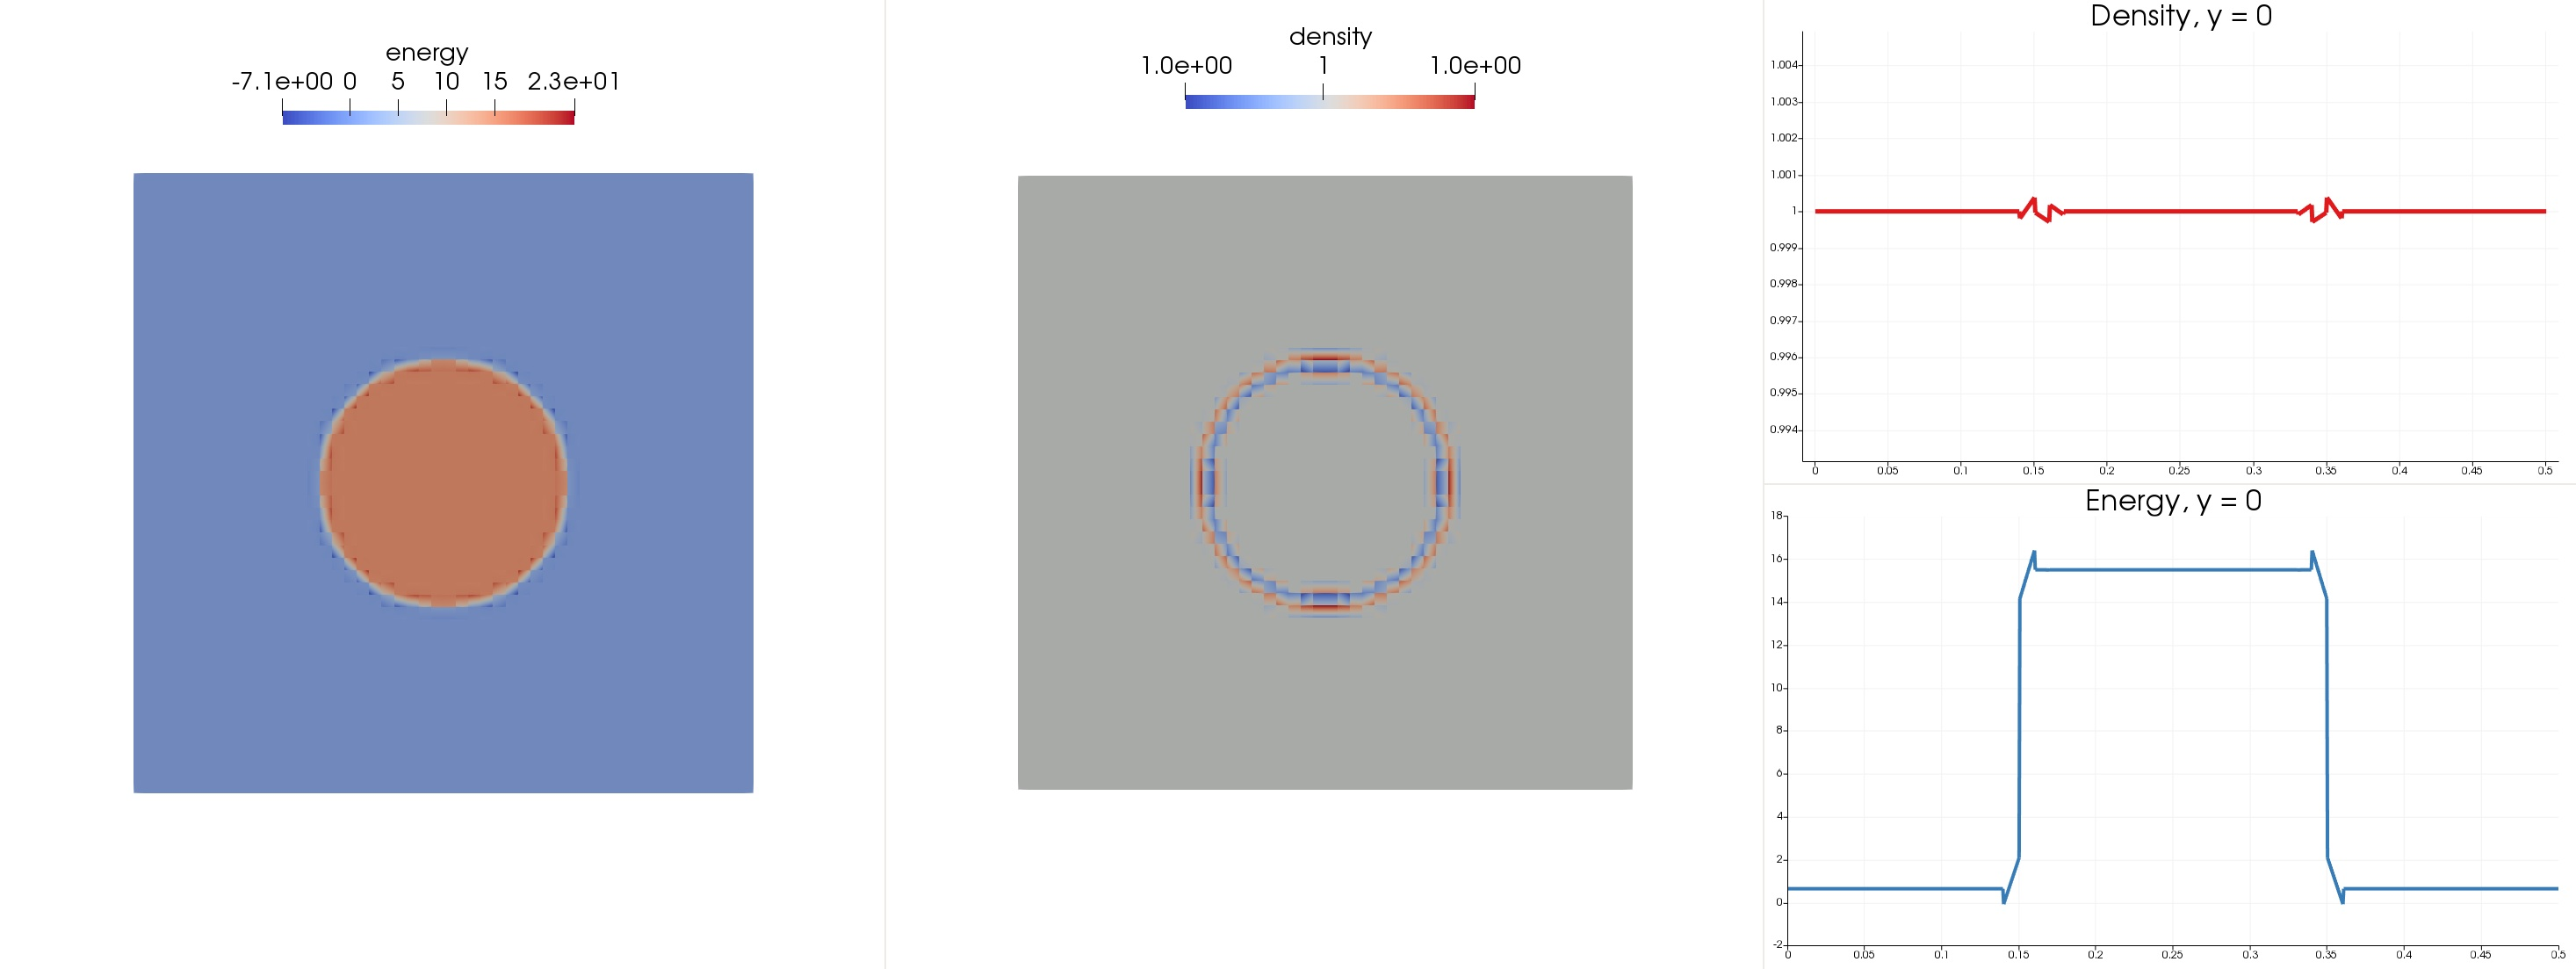
\includegraphics[width=0.82\textwidth]{img/limit/nl1.jpg}
		\end{center}
	\end{figure}\vspace{-12mm}
	\begin{figure}[H]
		\begin{center}
			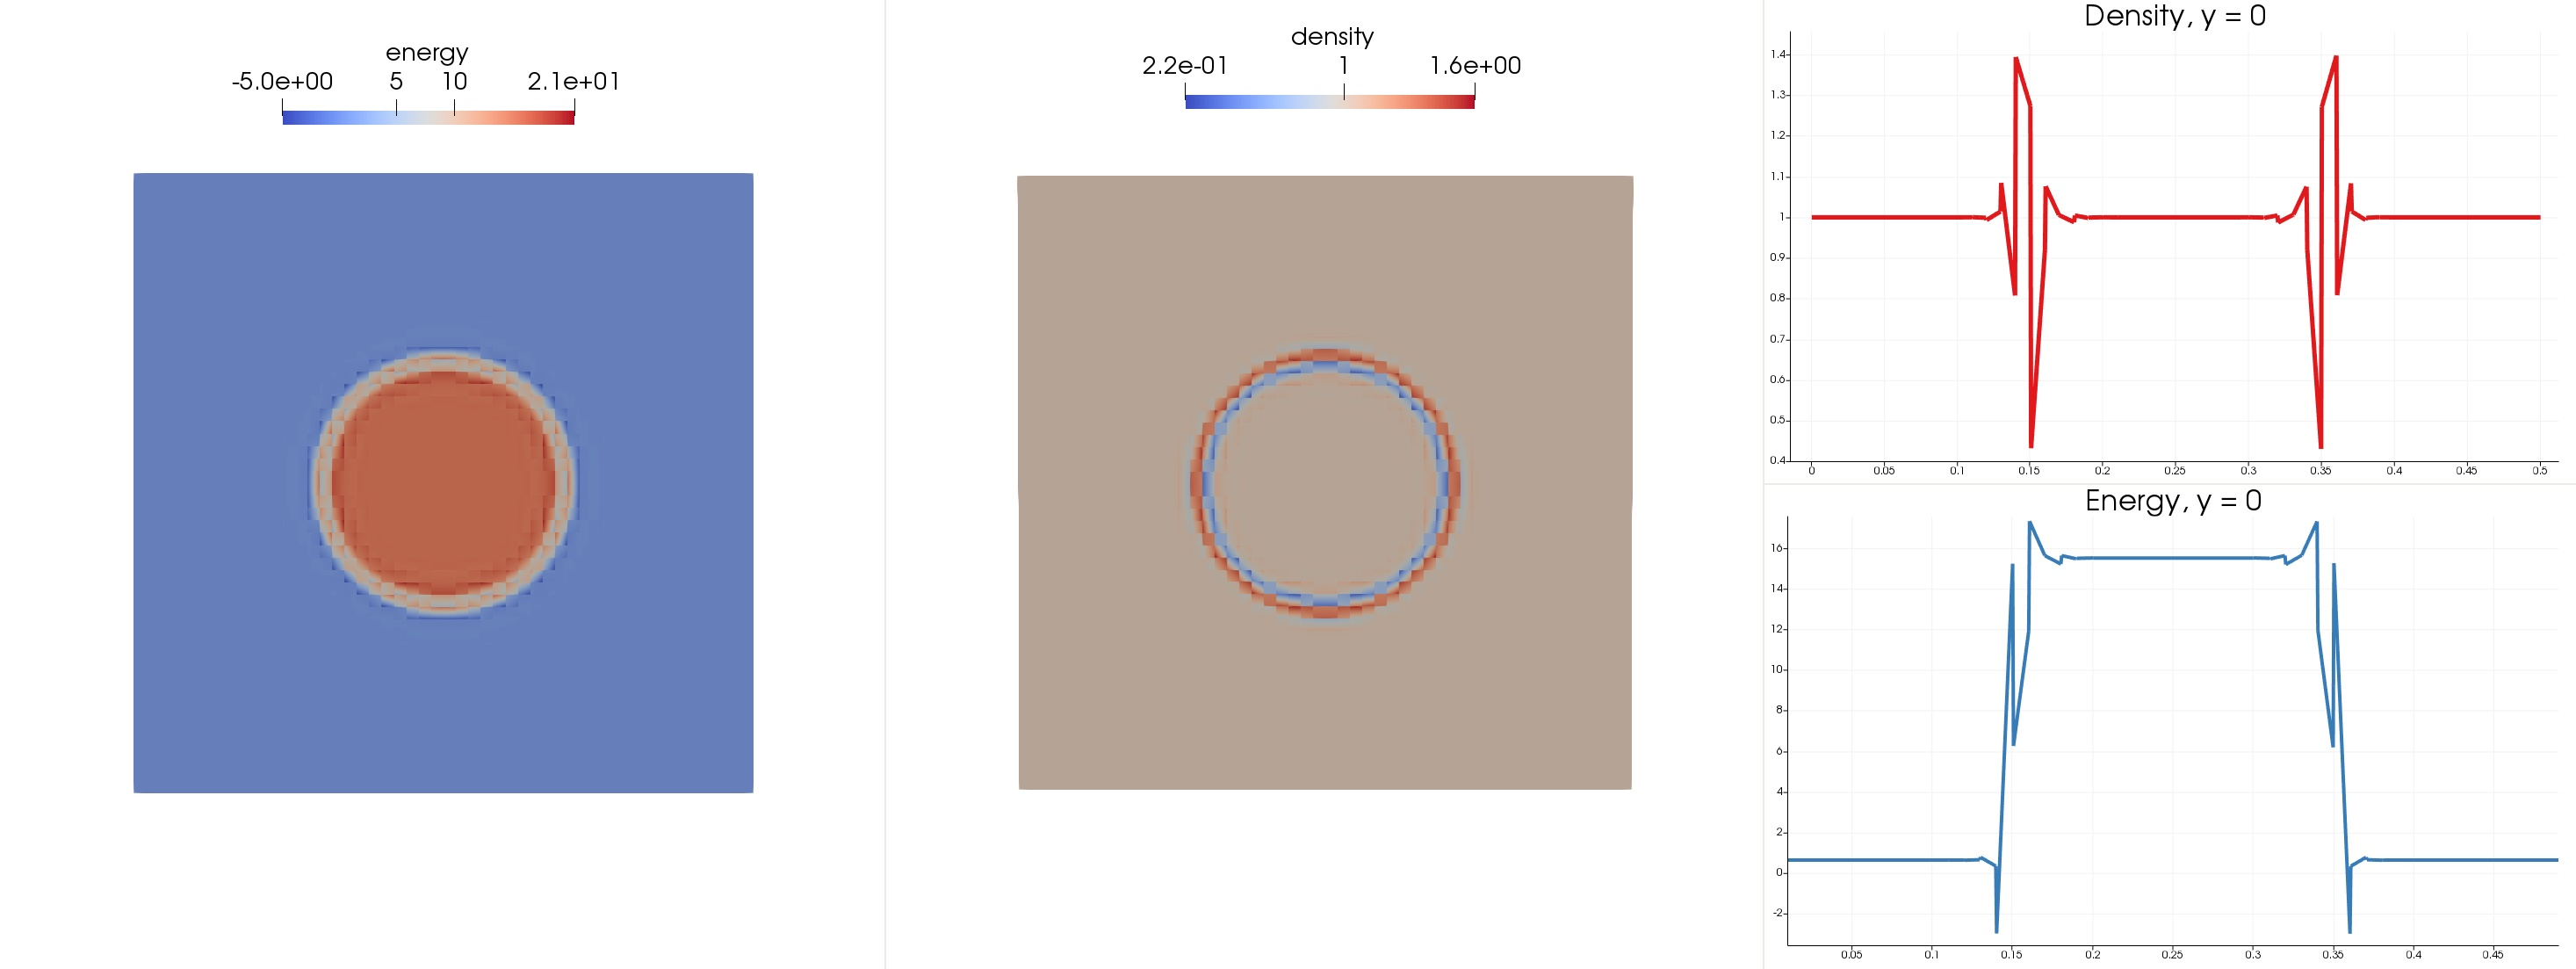
\includegraphics[width=0.82\textwidth]{img/limit/nl2.jpg}
		\end{center}
	\end{figure}\vspace{-12mm}
	\begin{figure}[H]
		\begin{center}
			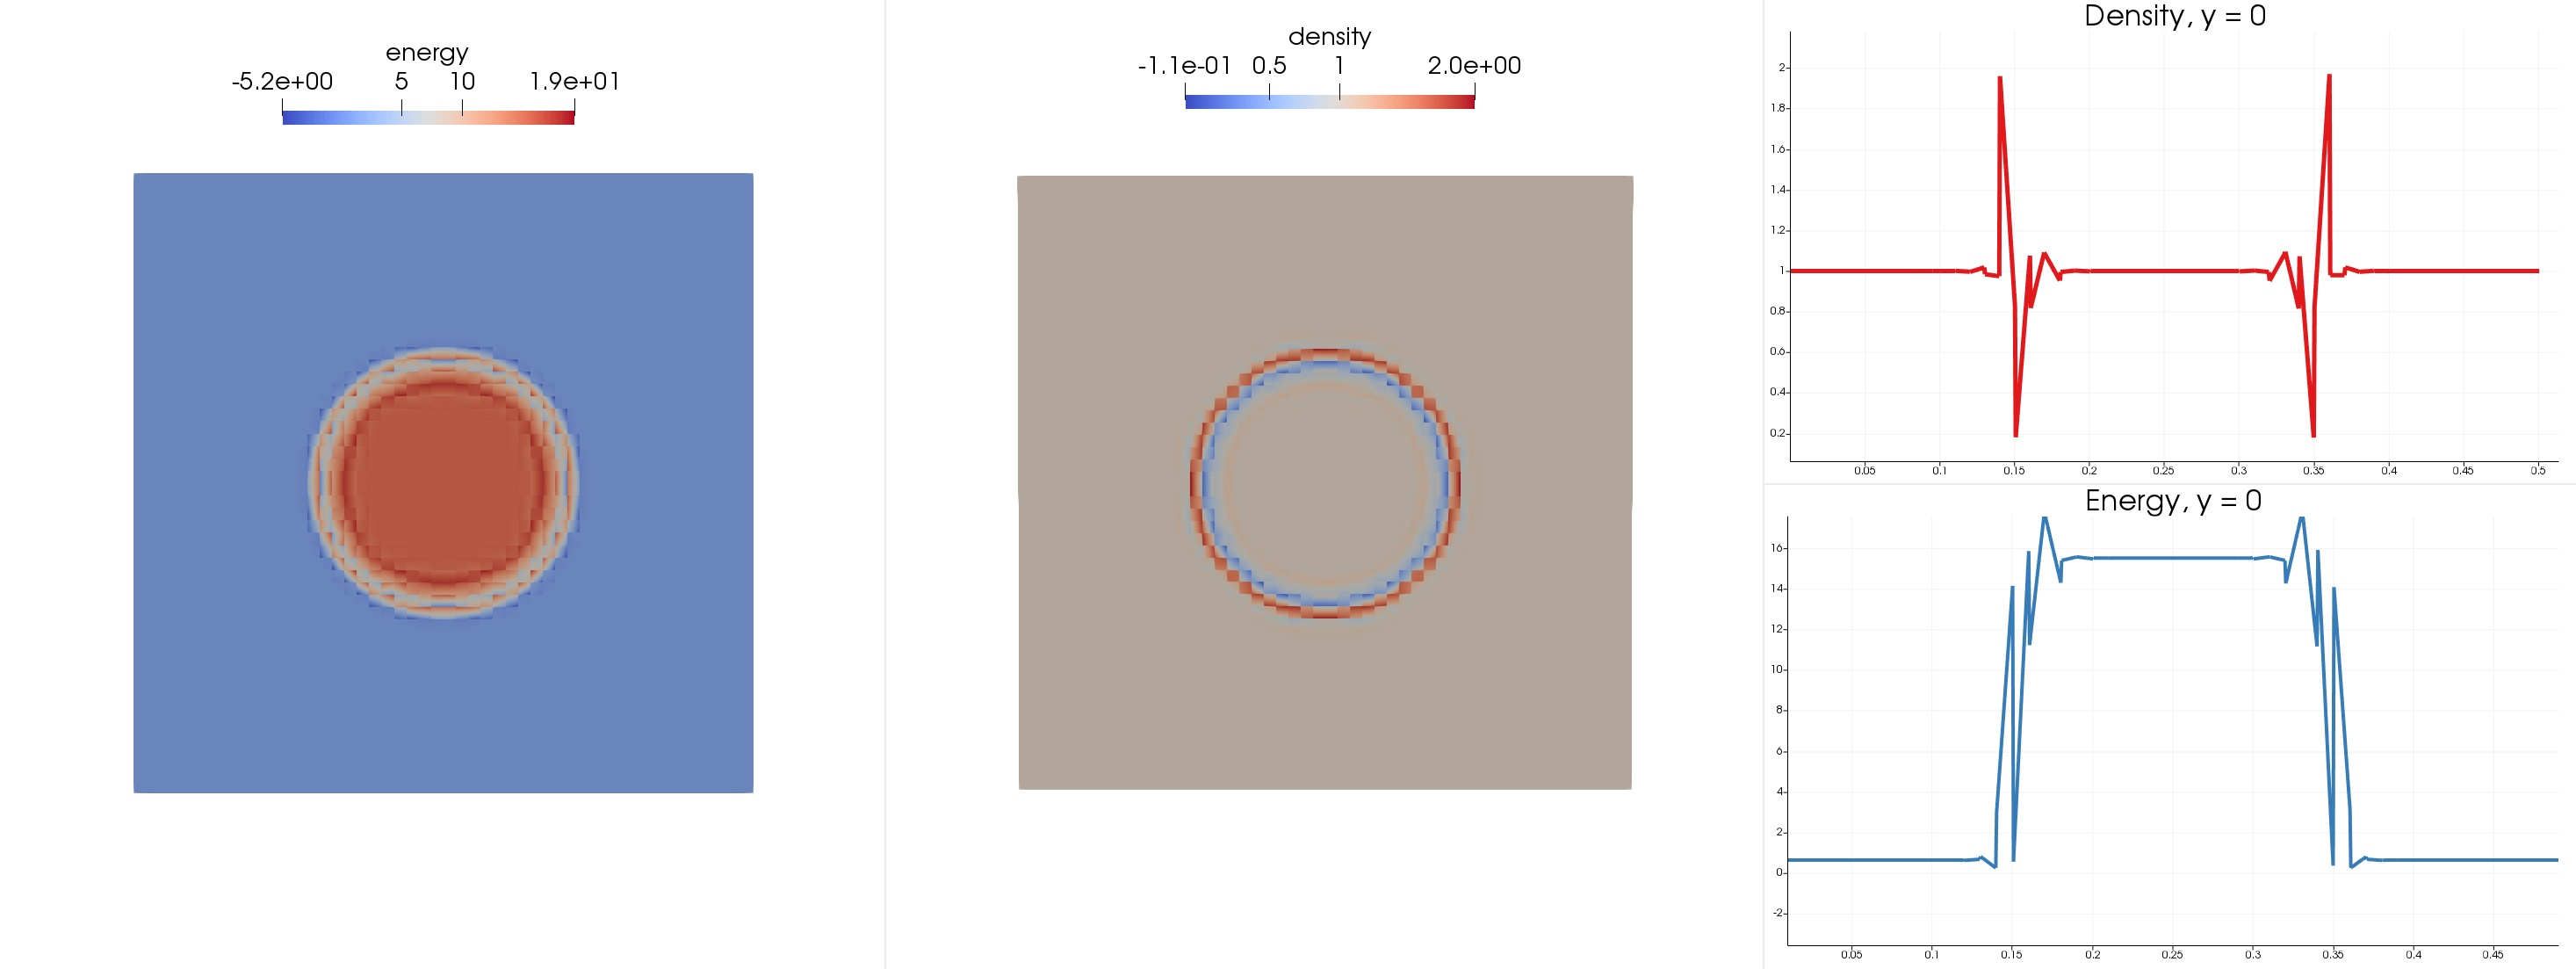
\includegraphics[width=0.82\textwidth]{img/limit/nl3.jpg}
		\end{center}
	\end{figure}\vspace{-12mm}
	\begin{figure}[H]
		\begin{center}
			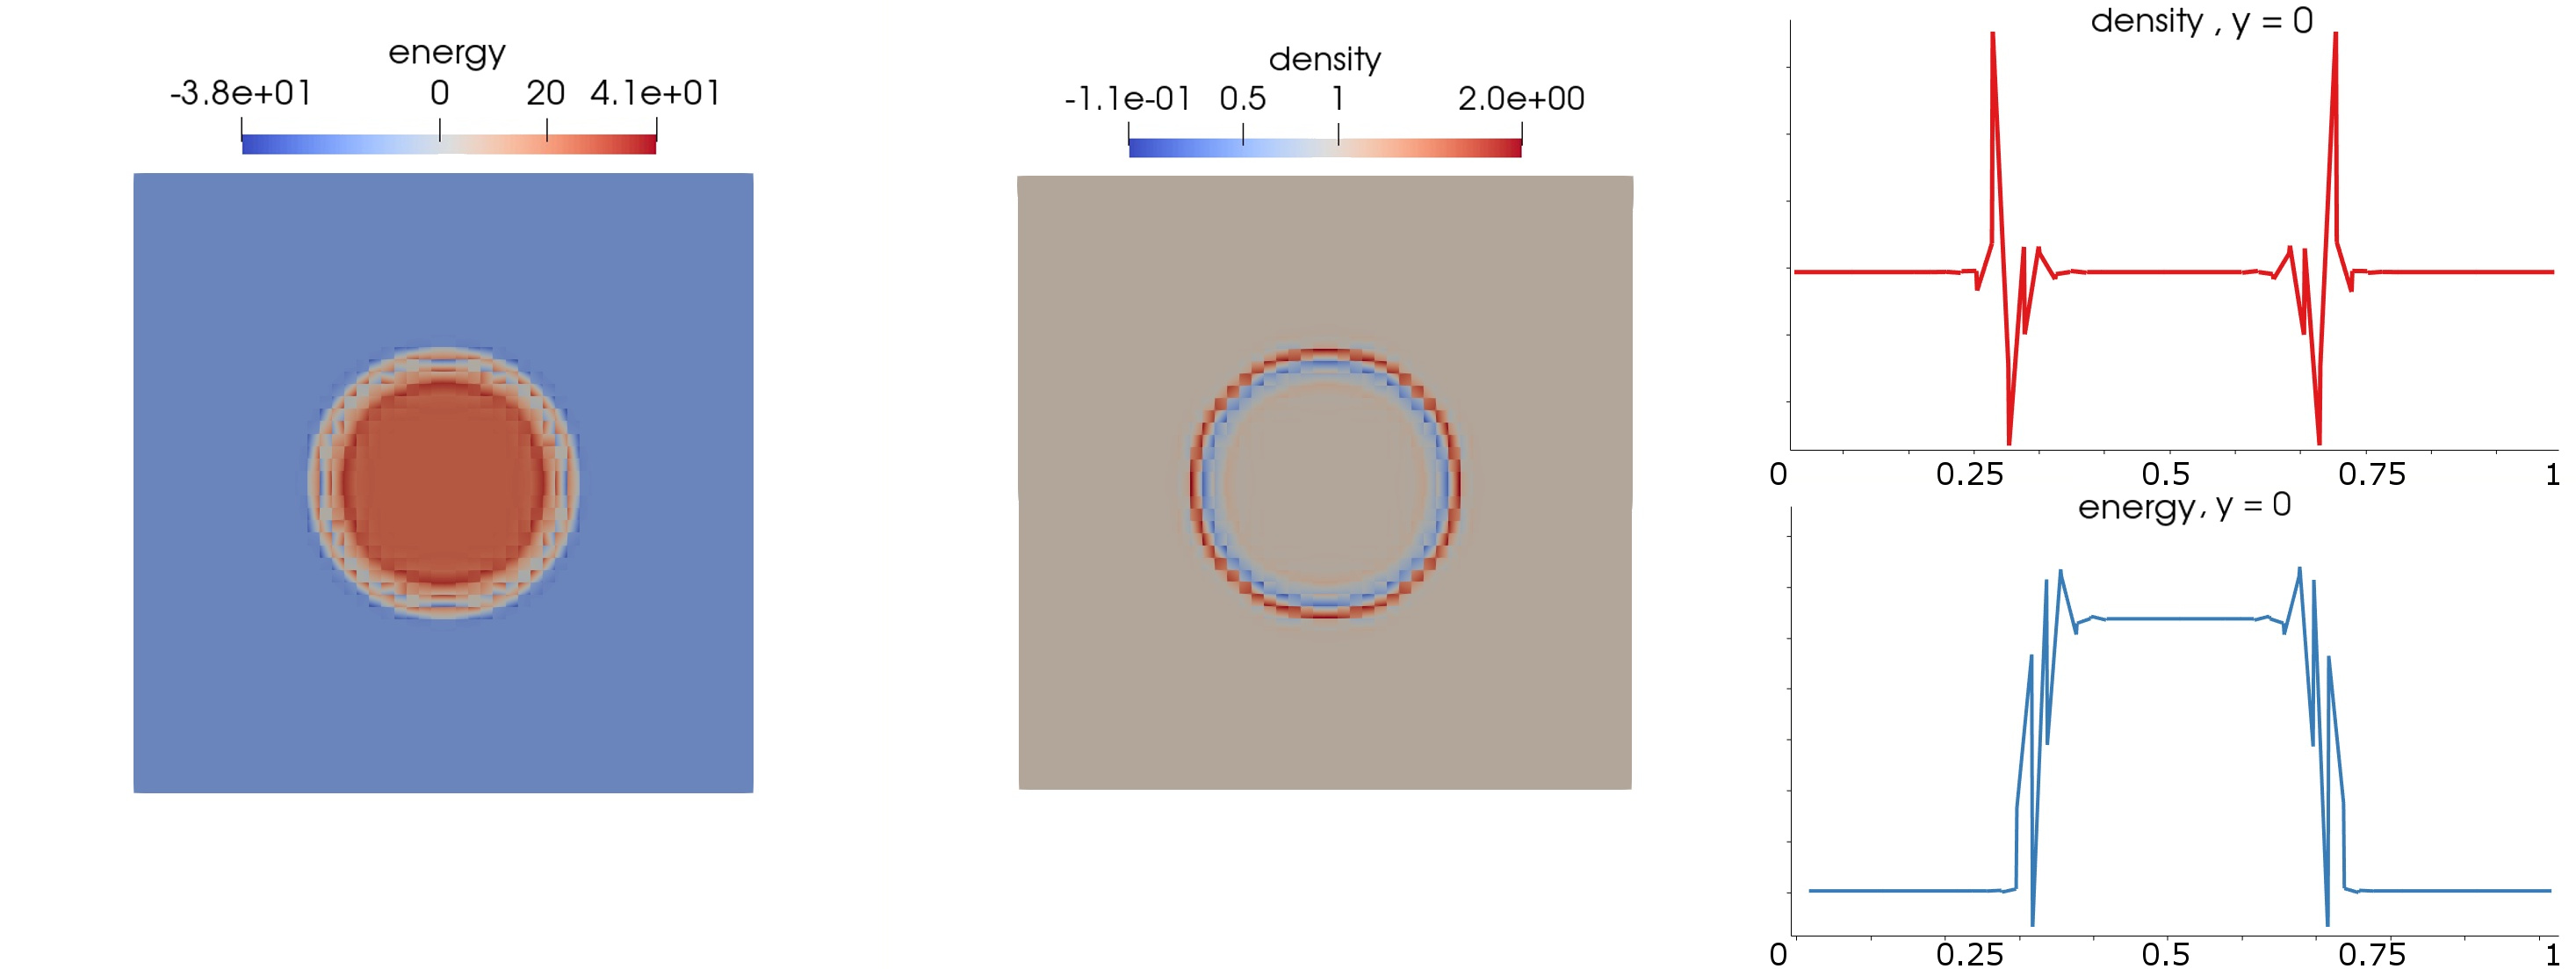
\includegraphics[width=0.82\textwidth]{img/limit/nl4.jpg}
		\end{center}
	\end{figure}\vspace{-12mm}
	\begin{figure}[H]
		\begin{center}
			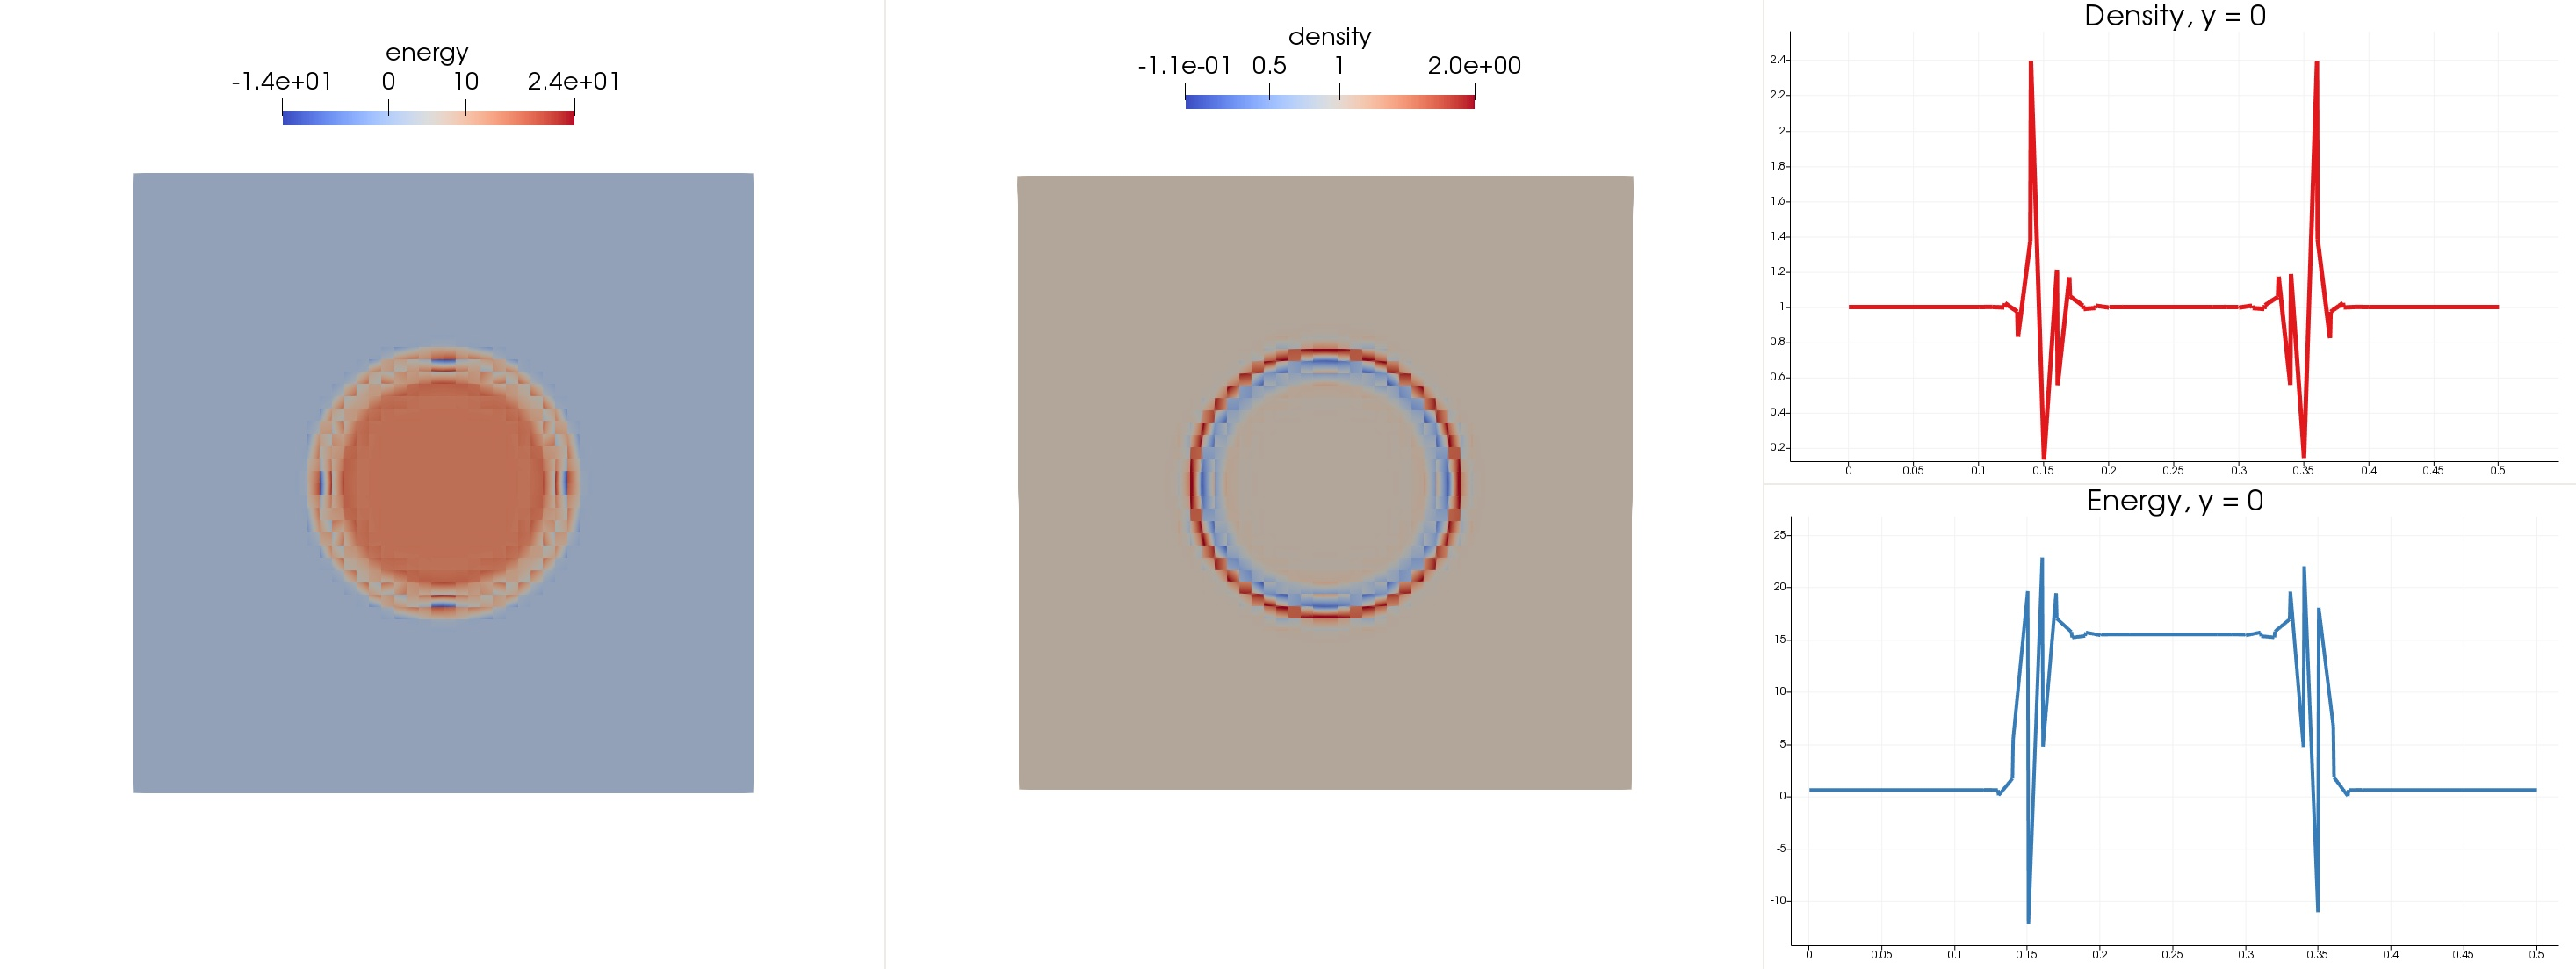
\includegraphics[width=0.82\textwidth]{img/limit/nl5.jpg}
		\end{center}
	\end{figure}\vspace{-12mm}
	\begin{figure}[H]
		\begin{center}
			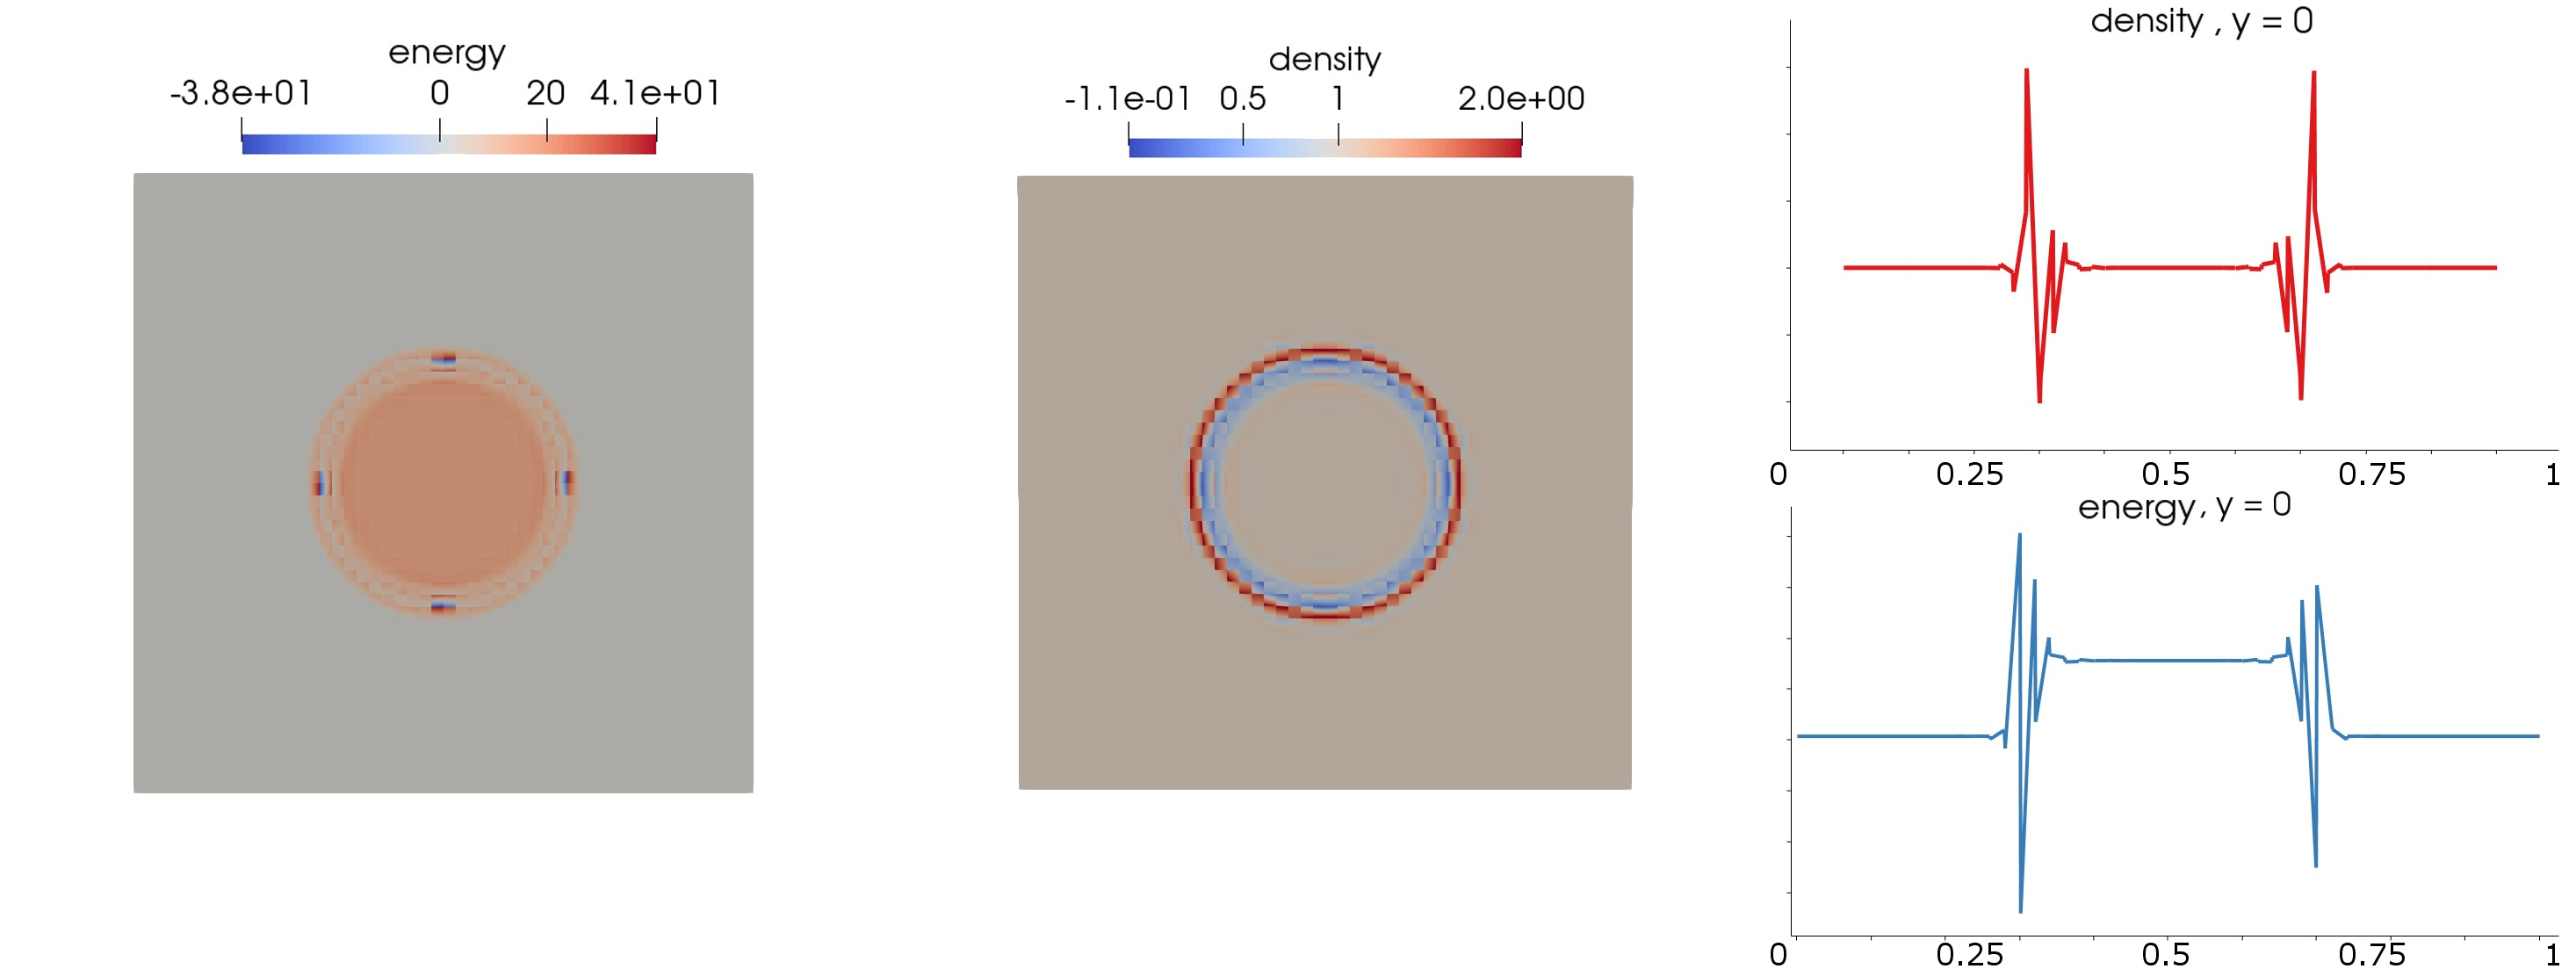
\includegraphics[width=0.82\textwidth]{img/limit/nl6.jpg}		
			\vspace{-4mm}
			\caption{Unlimited solution - Energy, density, and their values over line y = 0, the solution cannot progress beyond the last snapshot, as the oscillations are orders of magnitude larger than the physical solution}
		\end{center}
	\end{figure}
	
	\newpage
	
\begin{figure}[H]
		\begin{center}
			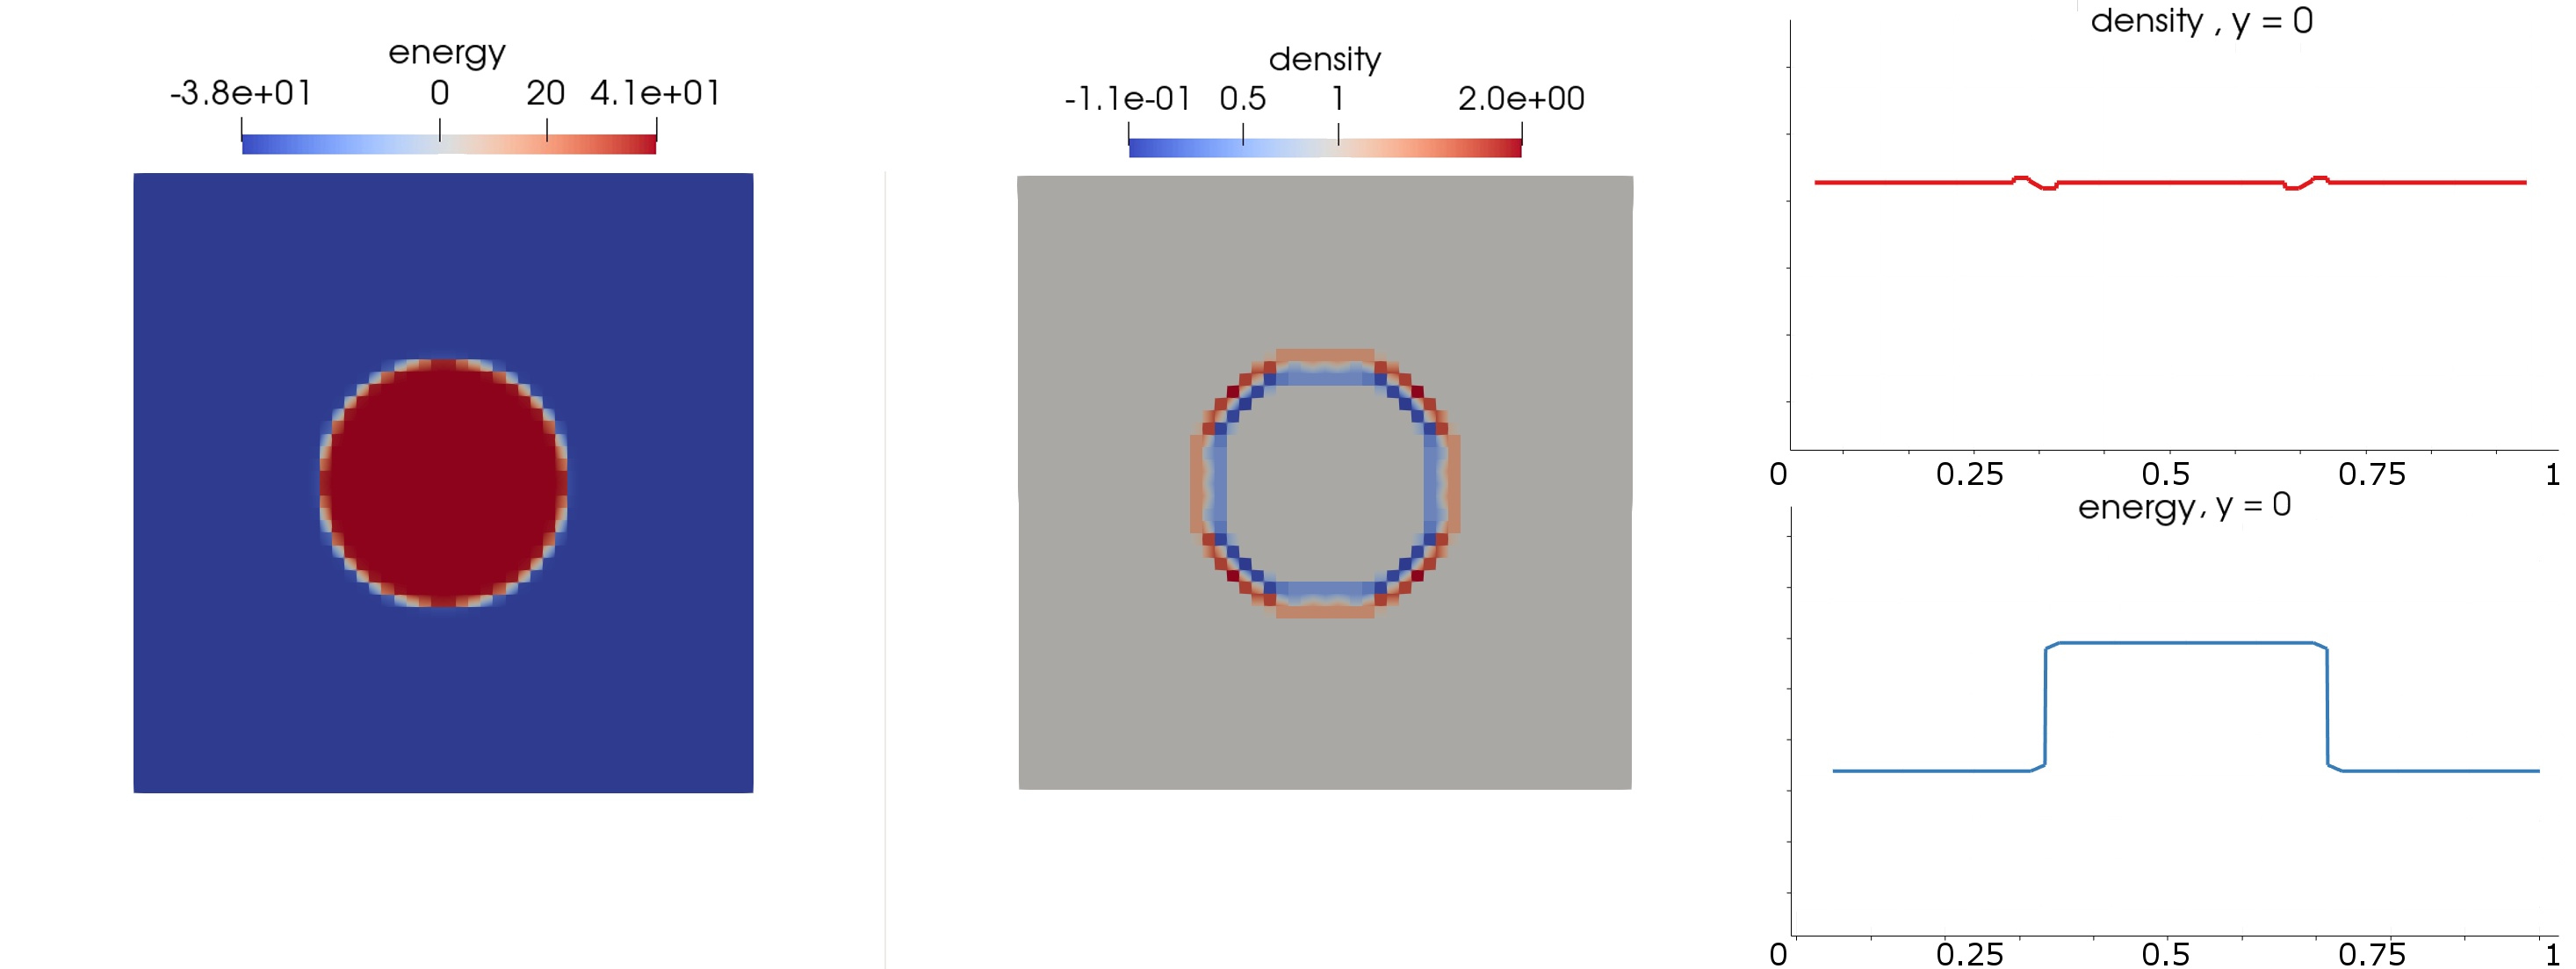
\includegraphics[width=0.82\textwidth]{img/limit/l1.jpg}
		\end{center}
	\end{figure}\vspace{-12mm}
	\begin{figure}[H]
		\begin{center}
			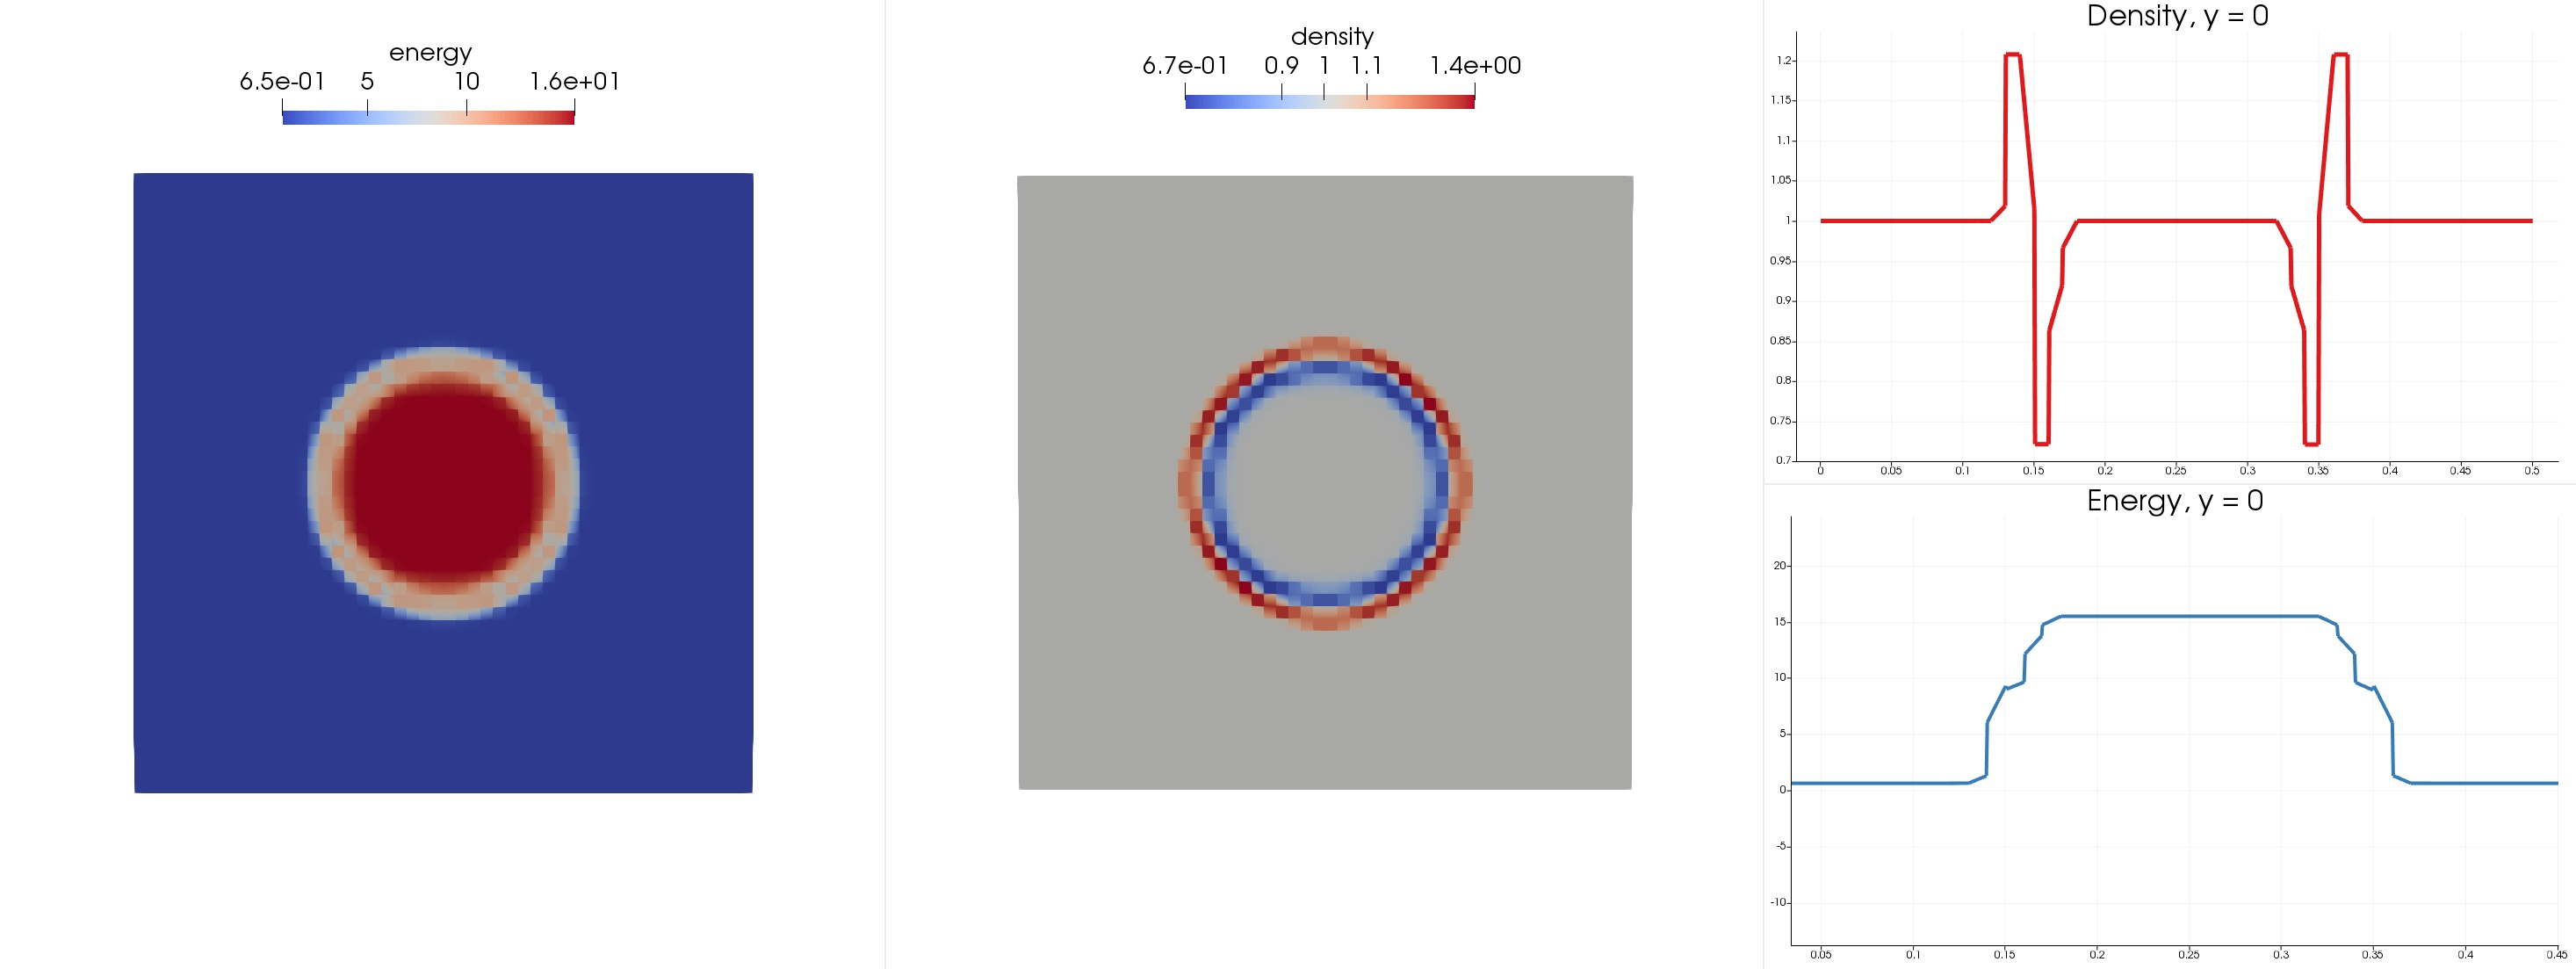
\includegraphics[width=0.82\textwidth]{img/limit/l2.jpg}
		\end{center}
	\end{figure}\vspace{-12mm}
	\begin{figure}[H]
		\begin{center}
			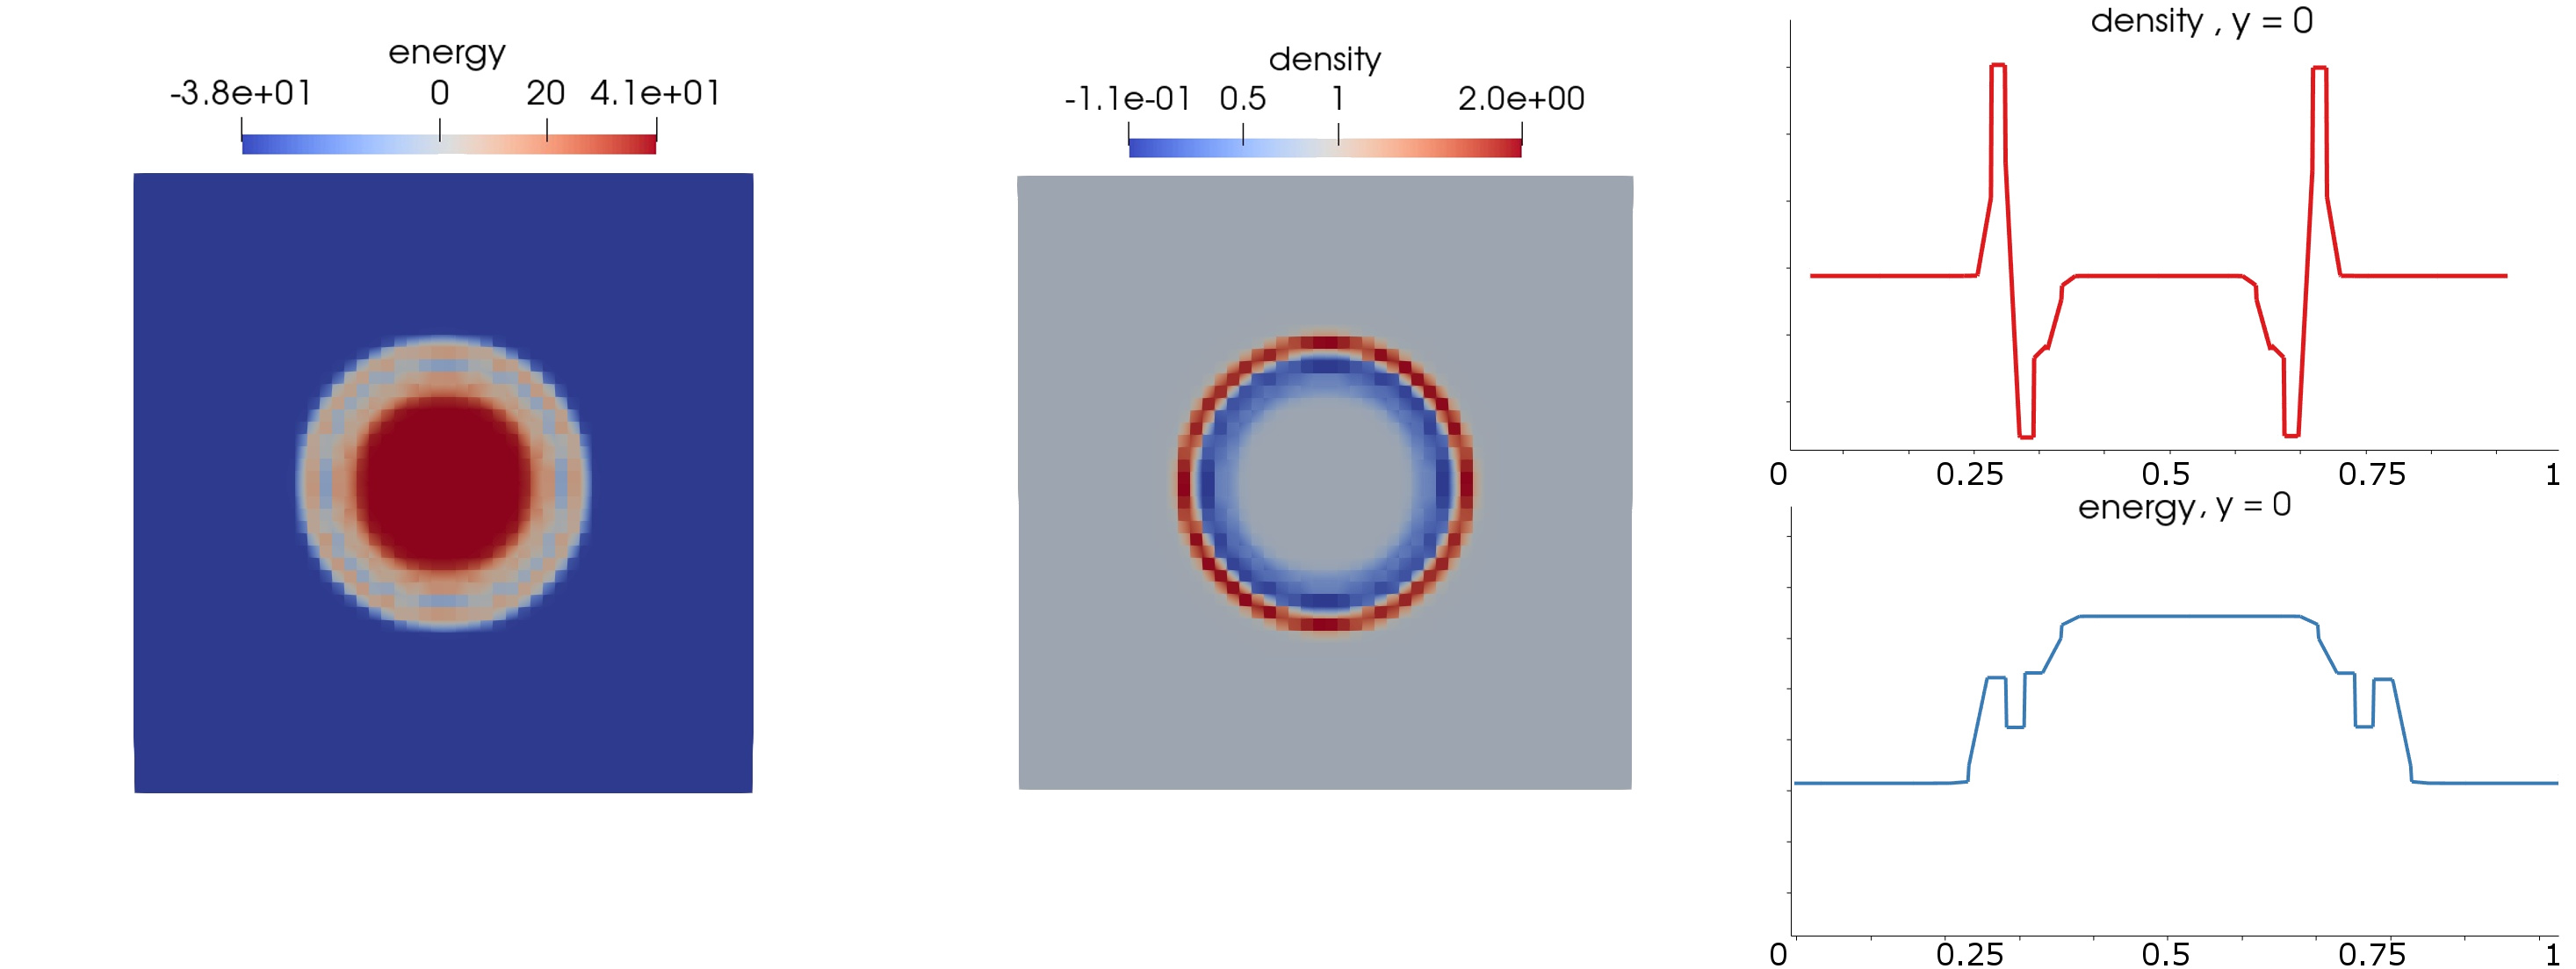
\includegraphics[width=0.82\textwidth]{img/limit/l3.jpg}
		\end{center}
	\end{figure}\vspace{-12mm}
	\begin{figure}[H]
		\begin{center}
			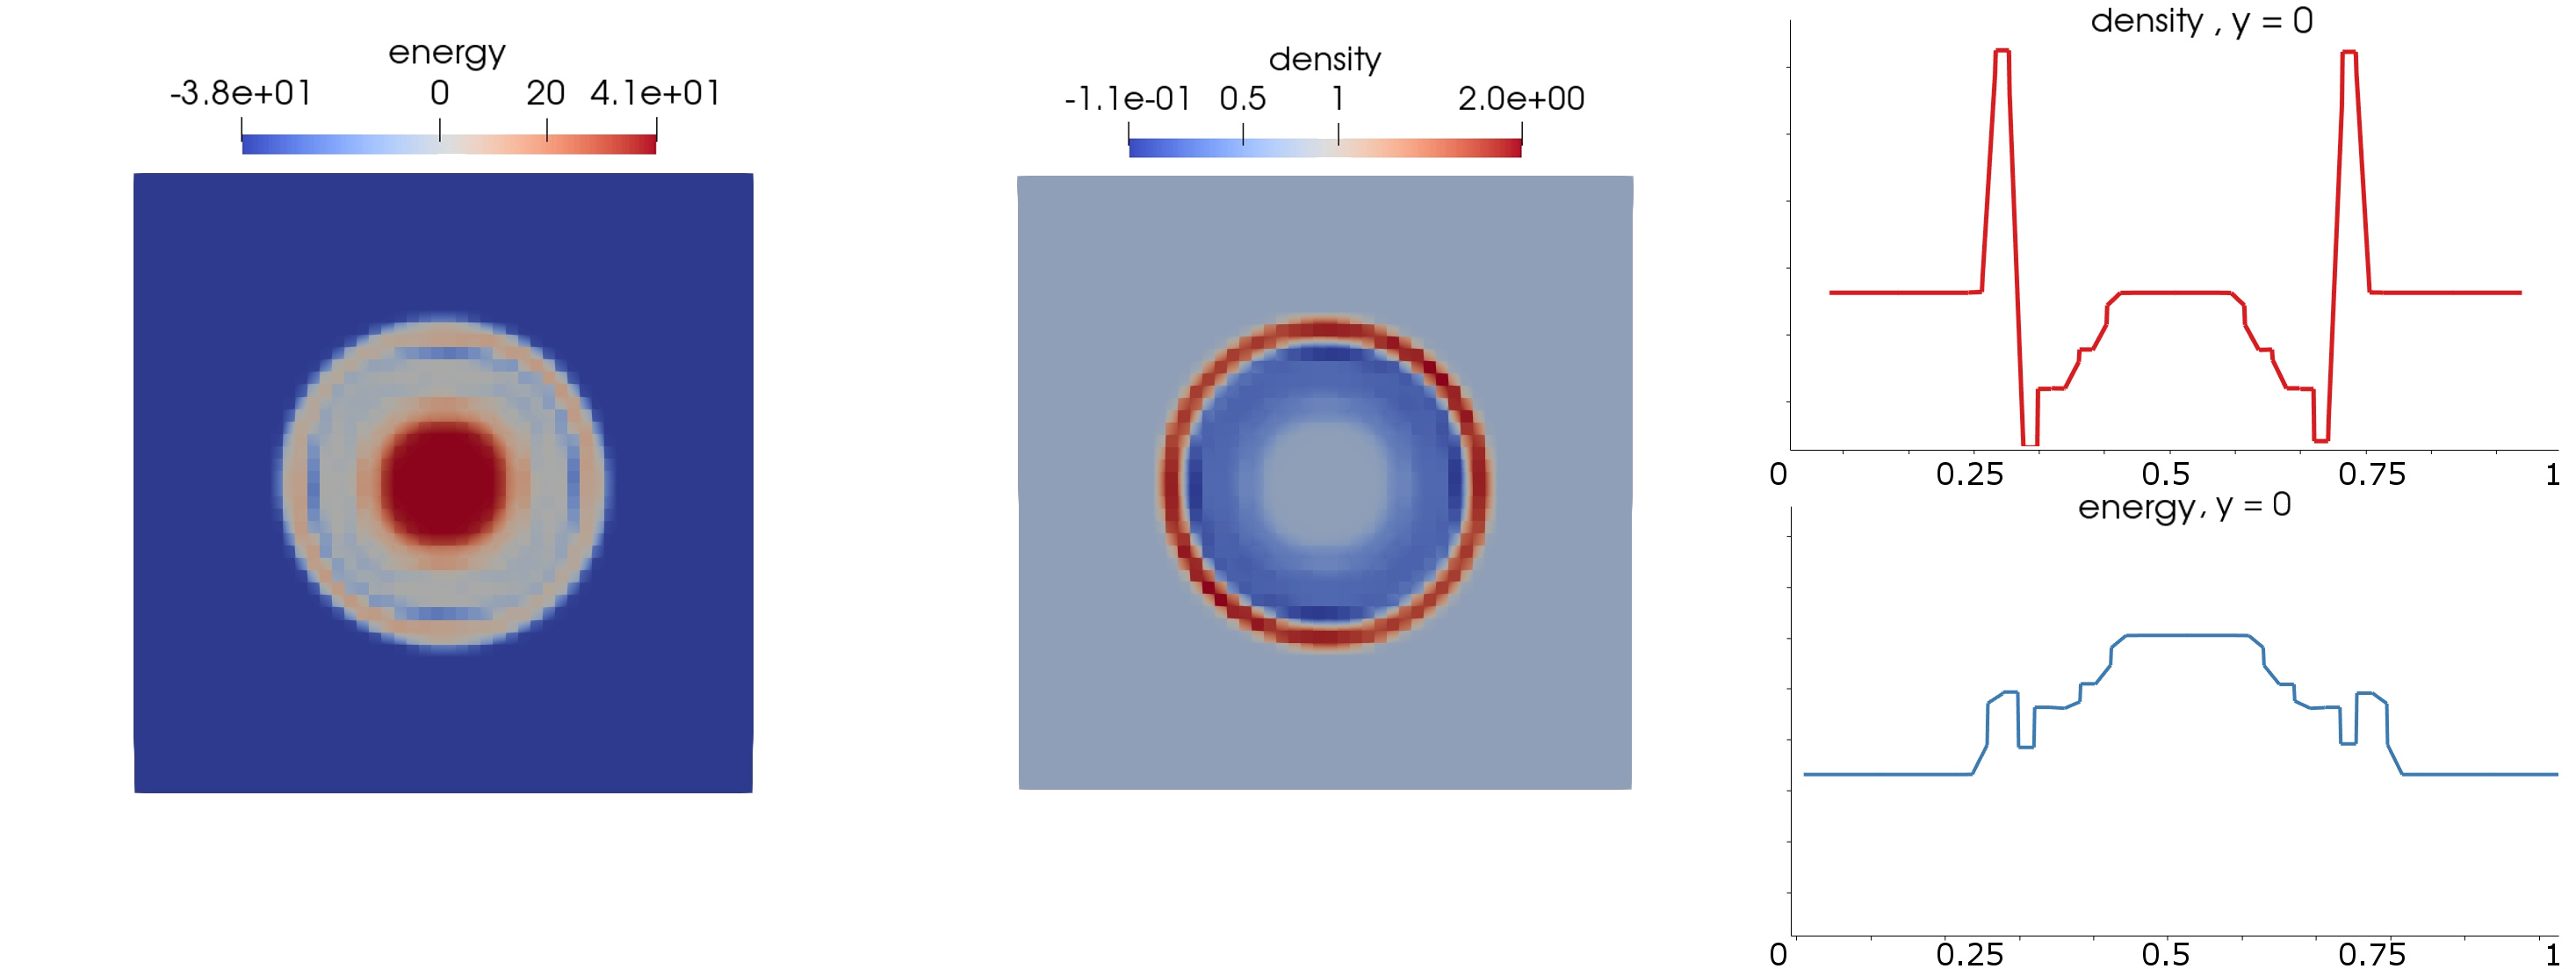
\includegraphics[width=0.82\textwidth]{img/limit/l4.jpg}
		\end{center}
	\end{figure}\vspace{-12mm}
	\begin{figure}[H]
		\begin{center}
			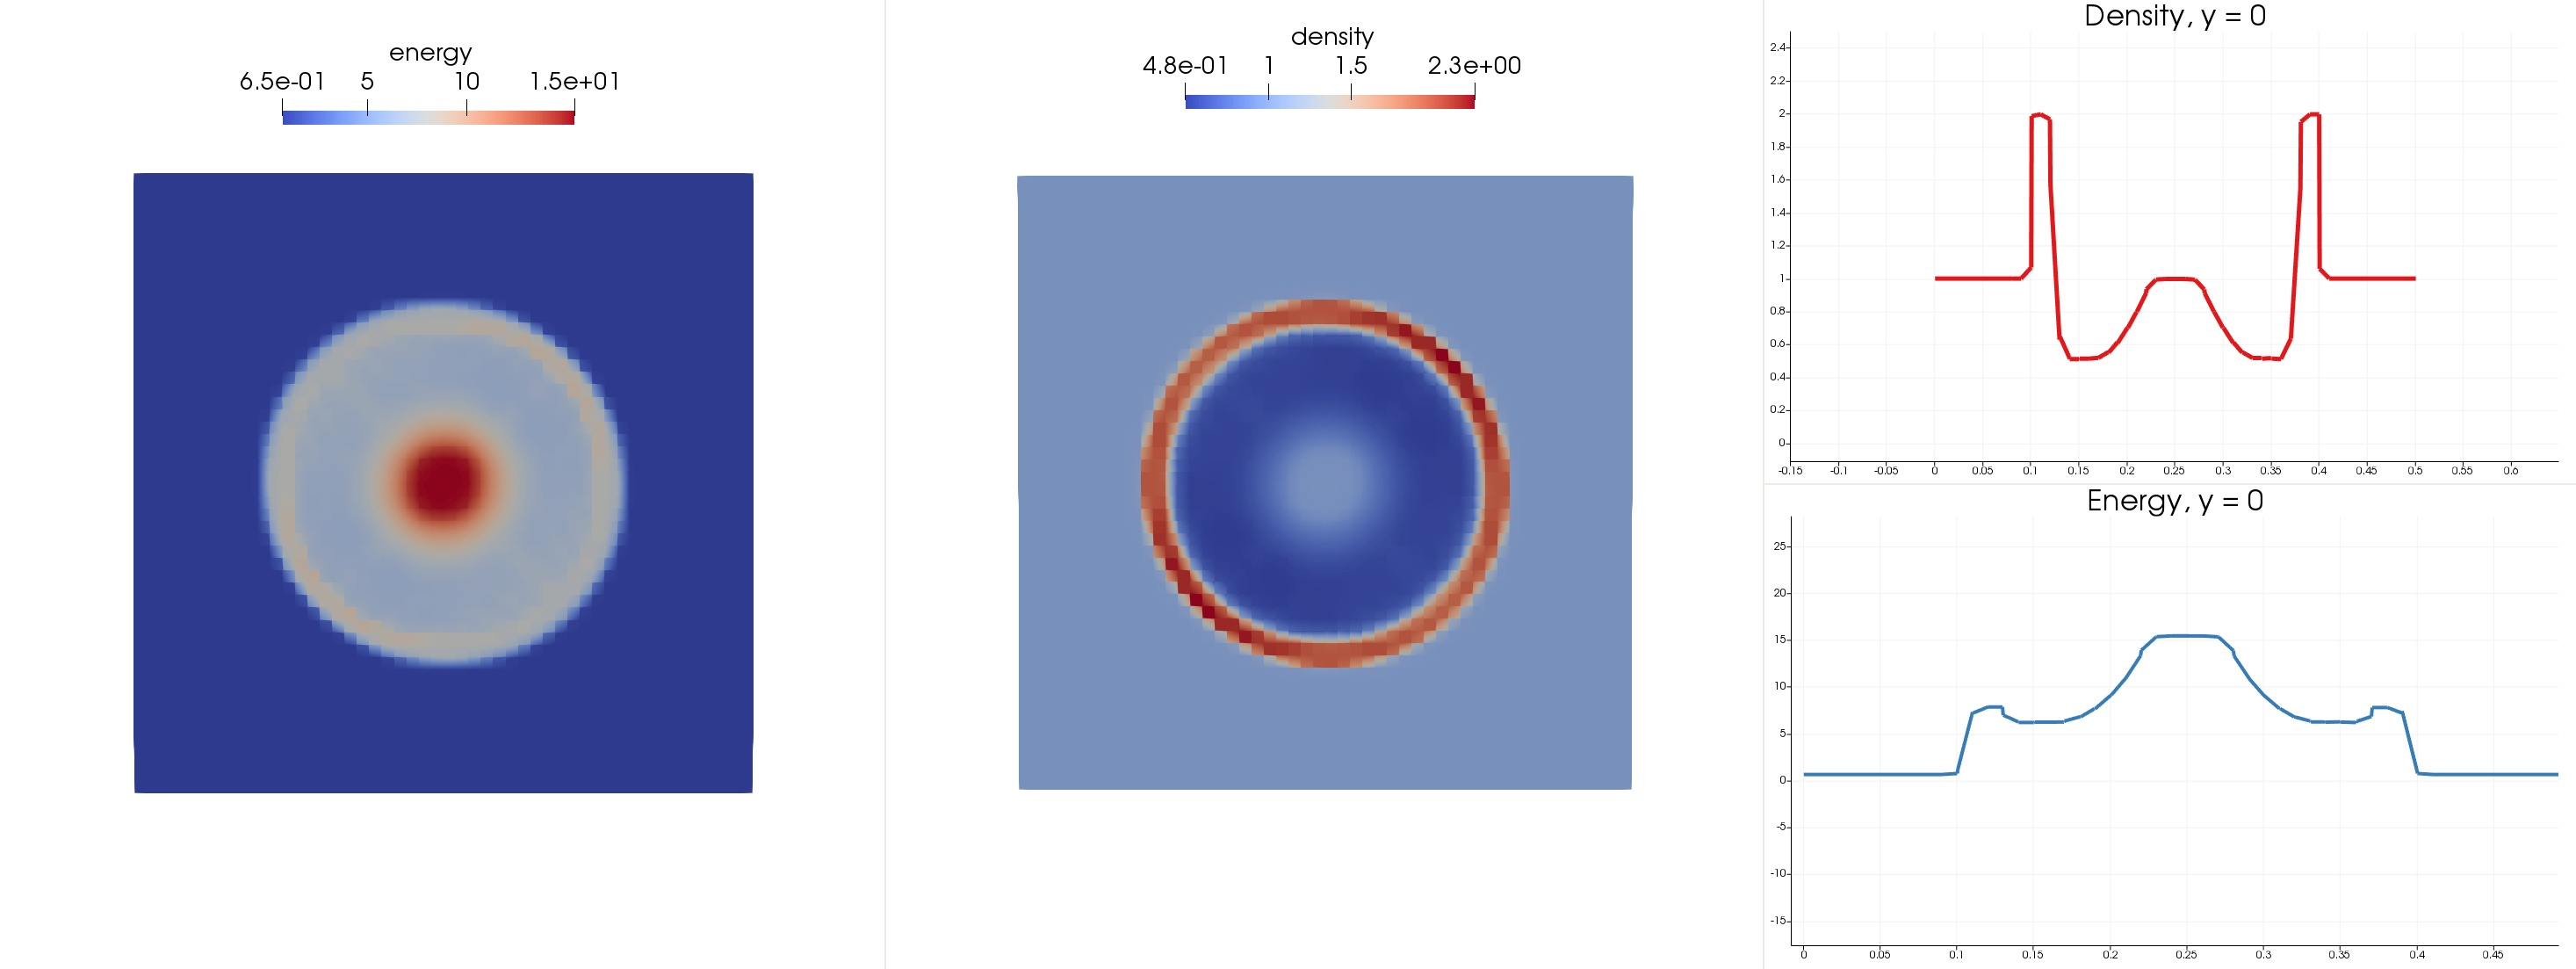
\includegraphics[width=0.82\textwidth]{img/limit/l5.jpg}
		\end{center}
	\end{figure}\vspace{-12mm}
	\begin{figure}[H]
		\begin{center}
			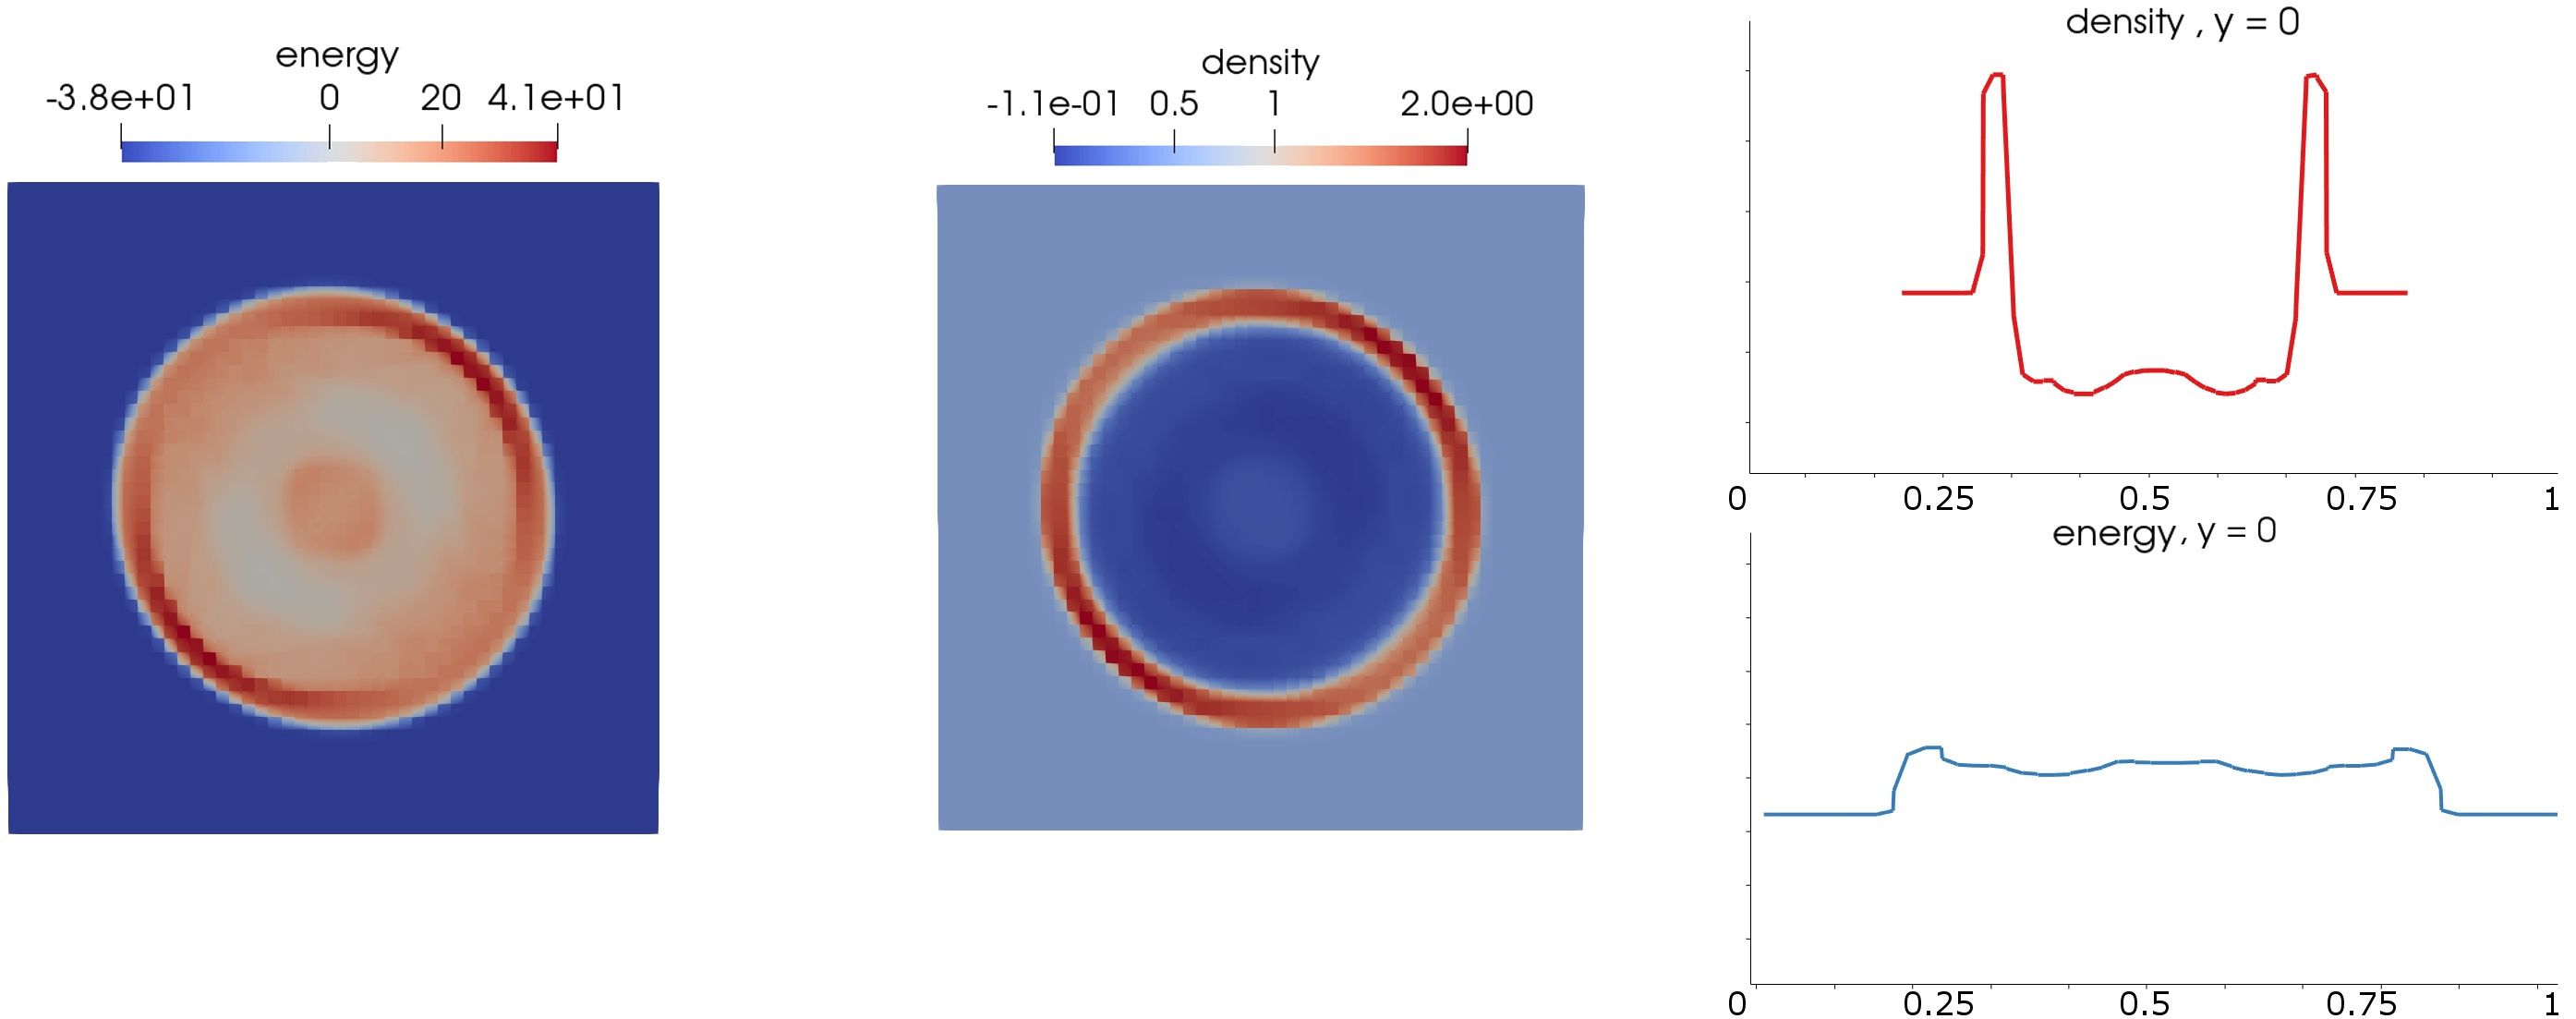
\includegraphics[width=0.82\textwidth]{img/limit/l6.jpg}
			\vspace{-4mm}
			\caption{Solution limited with Vertex-based limiter - Energy, density, and their values over line y = 0}
		\end{center}
	\end{figure}


%\section{Calculation considerations}
%
%\subsection{Stability}
%
%\subsection{Convergence}
%
%\subsection{Dissipation}

\section{Time-stepping and linearization}

\subsection{Time-stepping}
The simple time discretization scheme that we use in \cref{section:discreteProblem} allows us to simply implement the time-stepping in the following fashion:\\
\begin{algorithm}[H]
\textbf{    Set: }$y_0 =\ $ (initial solution)\\
\textbf{    Set: }$ts = 1 $ \# initial time step\\
\textbf{    Set: }$t = 0.00 $ \# initial time\\
    \# Loop over time steps\\
    \For{$;\ t < T;\ t = t+\tau,\ ts = ts + 1$}{
        \KwData{Solution from the previous time step $y^{ts - 1}$}
1.Call procedure \cref{algorithm:singleTimeStep} to obtain $A, b\lo y^{ts - 1}\ro$\\
2.Solve the problem $Ay^{ts} = b\lo y^{ts - 1}\ro\ $ \# See note below\\
3.(If necessary) postprocess $y^{ts}$ using \cref{algorithm:limiter}\\
4.Calculate updated value of $\tau$ using \cref{equation:CFLcond}\\
	 }
    \caption{Time-stepping procedure}
\label{algorithm:timeStepping}
\end{algorithm}
\paragraph{Note}
\label{note:solvers}
The step 2 (solving the algebraic problem) is of course a key point in the overall process. Because of its importance, the aim of this work is not to describe, or even implement an algebraic solver for this purpose. Many scientific teams have spent many years on publicly available open-source solvers that are usable by the software we develop for the purpose of solving the MHD phenomena. We use the existing solvers.

\section{Performance considerations}
Since eventually results are obtained by running a (distributed) program that implements the numerical methods, it is important to focus also on the performance aspects of the implementation, and not only on the numerical schemes. Plainly put, even a very efficient numerical algorithm can run on a computer a very long time, if not implemented properly.
\subsection{Parallelization}
\label{section:parallel}
To be able to perform any large scale calculations, we need to be able to utilize the performance of hardware at maximum. Being able to use modern, multi-core computers is an absolute must to achieve good performance, as the execution time when using parallel execution can decrease by a factor of corresponding to the number of cores - and modern machines have tens of cores available.

The parallelization is possible at several places in the overall algorithm \cref{algorithm:singleTimeStep}. But it makes most sense to parallelize the outer-most loop over elements, and over faces.

\paragraph{}
Another point for parallelization is the algebraic solver. As explained in \cref{note:solvers}, we rely on existing software packages for finding the solution of the algebraic system \cref{Alg} - all the used solvers support and heavily utilize parallelization.

\subsection{Vectorization}
Similarly as in section \cref{section:parallel}, the goal here is to be able to solve the discretized problem in the most efficient (fastest) way possible. One of the features that (modern) hardware offers is to employ vectorization instructions - i.e. unary or binary instructions that operate on $N, N > 1$ values (in case of unary instructions), or $N, N > 1$ pairs of values (in case of binary instructions) at the same time - the number $N$ depends on the capabilities of the CPU, and on the precision (single or double). On the hardware that was available to perform calculations for this thesis (and based on always-used double precision), $N = \left\{4, 8\right\}$, using such instructions requires both using them in the code (one has to specify that these instructions shall be generated explicitly), and having the compiler aware of these, and able to utilize them in the generated machine code - both compilers used for work on this thesis (GNU gcc, and Microsoft Visual Studio) support vectorization instructions (SSE, SSE2, AVX, AVX2).
\paragraph{}
Vectorization helps heavily with respect to CPU time spent on calculation. In the algorithm \cref{algorithm:singleTimeStep}, vectorized instructions are used in:
\begin{itemize}
    \item evaluation of the expressions $a_{lm} += JxW_{\bfj} \ a_{lm K \bfj}$
    \item evaluation of expressions $b_{l} += JxW_{\bfj} \ b_{l K \bfj}|_{face|volumetric}$
    \item calculation of $JxW_{\bfj}$
\end{itemize}

\subsection{Distribution}
As discussed in \cref{section:ditributedTria}, the \textit{domain decomposition} approach is taken to overcome the physical limitations (CPU physical size, RAM capacity, ...) of a single machine with shared memory.
\paragraph{}
This approach has several aspects, that are worth mentioning. The entire process of discretization of MHD equations (as well as any other system of PDEs) eventually leads to solving large (sparse) systems of linear equations, and then interpretation of the solution in terms of a global (defined on entire $\Omega$) function - that is a linear combination of the global basis functions with the solution of the linear problem being the coefficients of this linear combination. From this it follows, that distributing only the triangulation would not by itself lead to radical increase of the size of problems we can tackle, there are other points where the algorithms employed need to take distribution of data among processors into account:
\begin{enumerate}
	\item
		Distributed matrix and right hand side
		\begin{itemize}
			\item It is necessary for each processor to be able to utilize the memory on the node it physically belongs to when writing values of calculated integrals into the algebraic structure (see steps $a_{lm}\ +=...$, $b_{l}\ +=...$ of \cref{algorithm:singleTimeStep}).
			\item Distribution of the matrix is actually very important from the memory capacity perspective. It is typically the largest data structure (together with preconditioner) used in the entire implementation - regardless whether the used method is FEM, DGFEM, or Finite Volumes for example.
		\end{itemize}
	\item
		Distributed algebraic solver
	When the algebraic structures (the matrix and the right hand side) are completed, the sought solution must again be sought in a distributed manner, otherwise the added cost would be transferring algebraic data from all processors to a common one, where the solution would be sought. This is, however, a theoretical possibility, as the data structures used in the solution of the algebraic problem (decompositions, preconditioners, ...) are typically too large to be stored on a single processor anyway.
	\item
		Distributed solution
		\begin{itemize}
			\item Although it is quite obvious, it is noteworthy that as the algebraic structures are distributed, and so is the solution of the algebraic problem, the actual solution is again, distributed according to the domain decomposition.
			\item The distributed solution is the data structure that is most important from the perspective of the \textit{ghost cells} - illustrated in \cref{figure:ghost}, where for the distributed discontinuous Galerkin method, we need to be able to access the distributed solution values from all neighboring elements when performing numerical integration \cref{singleNumIntBface}.
		\end{itemize}
\end{enumerate}
\subsubsection{Message Passing Interface and deal.II}
For all distributed computing purposes in this work, deal.II implementation of the Message Passing Interface (MPI) was used. MPI is a specification for a standard library for message passing for the purposes of distributed computing, and was originally introduced in \cite{mpi}. The library deal.II (\cite{deal}) offers wrappers for low-level MPI functions, that are utilizable in the implementation of the methods of this work.
